
\chapter{Beyond Ethnicity: Historical States and Modern Conflict}
% \author[1]{Marius Swane Wishman} \author[1]{Charles Butcher}
% \affil[1]{Department of Sociology and Political Science, NTNU} \date{}

%\begin{center} Word count: \end{center}

\begin{abstract} Historical states, be they sprawling empires or nominal vassal
	states, can make lasting impressions on the territories they once
	governed. We argue that more historical states located within the
	borders of modern states increase the chance of civil conflict because
	they: (1) created networks useful for insurgency, (2) were symbols of
	past sovereignty, (3) generated modern ethnic groups that activated
	dynamics of ethnic inclusion and exclusion, and (4) resisted western
	colonialism. Using new global data on historical statehood, we find a
	robust positive association between more historical states inside a
	modern state and the rate of civil conflict onset between 1946-2019.
	This relationship is not driven by common explanations of
	state-formation that also drive conflict such as the number of ethnic
	groups, population density, colonialism, levels of historical warfare,
	or other region-specific factors. We also find that historical states
	are more likely to be conflict inducing when they are located far from
	the capital and in poorer countries. Our study points to unexplored
	channels linking past statehood to modern day conflict that are
	independent of ethno-nationalist conflict and open possibilities for a
	new research agenda linking past statehood to modern-day conflict
	outcomes.

\end{abstract}

\bigskip \keywords{Artificial states, civil conflict, historical states, state
entities, state formation, civil war, ethnic conflict, pre-colonial states}

\pagebreak


\section{Introduction}

%{{{ 
Hundreds of independent states existed in the 19th century that no longer appear on political maps, many extinguished by colonialism. Some
countries encompass many of these historical states while others contain few.
Studies reach differing conclusions on whether these historical states are a
source of conflict or stability in the modern world. Some find that prior
statehood (often labelled pre-colonial) facilitates peaceable solutions to
latent ethnic conflict \citep{Depetris-Chauvin2016, Wig2016}, while others find
that they can leave legacies of ethnic tension and war \citep{Besley2014,
Paine2019, Englebert2000, Alesina2003}. 
%}}}

We focus on the national-level effects of variations in the number of historical
states that modern states encompass. We label these states `Historical State
Entities' (HSEs) throughout the paper. We argue that states with more HSEs
within their modern borders experience more internal conflict onsets because
HSEs left behind social networks and symbols of sovereignty that were useful for
collective action, provided the raw material for ethnic claims making in the
post WWII period and resisted colonialism before independence and state
consolidation after. We test this theory with new measures of the number of HSEs
that existed in modern-day states from 1816-1939, finding that more HSEs
are positively correlated with civil conflict onsets between
1946-2019, an association that is not explained or mediated by more politically
relevant ethnic groups or excluded ethnic groups in the modern period. This
suggests that historical states are linked to conflict independently of their
impact on or through modern ethnic power relations that are the focus of most
research on the modern legacies of historical states \citep{Paine2019, Wig2016}.
Moving `beyond ethnicity' to understand how political topologies from the past
shape conflict may lead to new insights \citep{Herbst2014, Blaydes2013, Mazzuca2021}. We
suggest further research on the symbolic legacies and mobilization
infrastructures left behind by HSEs as a useful way forwards \citep{Ahram2019}. 

\section{Contribution}

This study makes three contributions to the existing literature on the legacies
of historical states and internal armed conflict. First, many studies assume
that prior statehood impacts conflict through relations between modern ethnic
groups and the state \citep{Englebert2002, Paine2019, Wig2016}, or measure prior
statehood with proxies of ethnic centralization. While incorporating these
important insights, we advance the field by highlighting mechanisms through
which historical states can influence conflict independent of ethnicity, and by
drawing on a global dataset of independent \textit{states} rather than ethnic
groups. The pre-colonial political landscape was certainly populated by ethnic
groups \citep{Murdock1967}, but it was also populated multi-ethnic empires. A
focus on ethnic groups can’t tell us about the legacies of the Sokoto Caliphate,
for example, which was a multi-ethnic empire overlapping with dozens of ethnic
groups in the oft utilised ``Murdoch Map''. Moreover, states often made modern
ethnic groups. There is, for example, little evidence of an ``Achenese'' ethnic
identity before the 20th century \citep{Aspinall2009}. This ``ethnic group'' is
a product of the Achenese Sultanate, which survived up to the beginning of the
20th century as an independent state before it was colonized by the Dutch and
incorporated into Indonesia (see also \citep{Wimmer2018}). 

Even if we grant the assumption that states and ethnic groups are coterminous,
it breaks down outside of Africa and is, therefore, a poor conceptual foundation
upon which to estimate the \textit{global} impacts of historical statehood.
States in South Asia and Southeast Asia were not strongly ethnic states. Studies
of historical legacies outside of Africa focus on empires and states
\citep{Acemoglu2011, Grosjean2011}, violent events \citep{Grosfeld2013},
economic systems and change \citep{Banerjee2005, Nunn2011}, or regional potentates \citep{Mazzuca2021}, not ethnic groups.
The Mughal and Maratha empires ruled ethnic groups, but neither was an
``ethnic'' state, nor was the Ottoman empire \citep{Richards1995, Ramusack2004,
Gordon1993}. Continuing from the assumption that we can study historical
statehood by studying ethnic groups, therefore narrows the scope for comparative
analysis.

Second, existing studies of historical \textit{statehood} are based on
incomplete datasets or regionally limited samples \citep{Besley2014,
Depetris-Chauvin2016, Dincecco2019, Michalopoulos2016, Nunn2008}. Most studies
in international relations use registers of states with in-built European biases
that exclude states in Africa, the Middle-East and Asia \citep{Sarkees2010,
Gleditsch1999}. There were hundreds of states in these regions in the 19th
century, but they are elided because datasets often pin “statehood” to
recognition by one or multiple European powers, usually England and France. For
some non-Western states, Europeans were simply not the most relevant
international actors. The French were a small, distant, coastal trading enclave
in the eyes of the massive Sokoto Caliphate in West Africa in 1816. The Oyo
Empire and Borno Emirate were more important regional powers. Moreover,
Europeans did not recognize some states for strategic reasons, especially if
they intended to conquer them \citep{Teorell2017}. The political map of the
globe, according to these datasets, is blank for swathes of Africa, Asia and the
Pacific. We use a global dataset of prior-statehood that is more comprehensive
than existing registers and does not select on matches with prior or modern
ethnicity \citep{Butcher2020}, allowing us to test -- rather than assume --
links between historical states, ethnic groups and modern conflict in addition
to mechanisms that do not strongly emphasise ethnicity. 

Finally, we contribute to the literature on `artificial states'
\citep{Alesina2011, Englebert2000, Herbst2014, Clapham1996}, by developing a
measure of state artifice that is more consistent with existing
conceptualizations. `Artificial states' are states that overlap poorly with the
pre-existing topology of statehood \citep{Alesina2011, Herbst2014}. Our measure
of the number of HSEs that existed on the territory
of a modern state between 1816 and 1939 more directly captures the overlap
between modern borders and past state structures than existing measures that
rely upon the `straightness' of modern borders \citep{Alesina2011} or the
variance in pre-colonial ethnic centralization \citep{Englebert2002}. 

    
\section{Theory}

\subsection{Historical state entities}

Our main argument is that countries with more historical state entities (HSEs)
within its borders experience more internal armed conflict onsets than countries
with fewer HSEs. HSEs are states that existed in the past that may or may not
exist in the modern international system. For convenience and consistency with
our measurement strategy below, `modern' is the period after the Second World
War and `historical' is the period before 1939 and the Second World War, which
was followed by the United Nations, decolonization and the modern-state system
as we know it today. 

Our definition of `statehood' comes from the International Systems Dataset (ISD)
\citep{Butcher2020}, which adopts a `thin' definition. States are
political entities with a population of at least 10,000, autonomy over a
specific territory and sovereignty that is either uncontested or acknowledged by
the relevant international actors. ISD states have a baseline level of
administrative structure, population and independence with the capacity to
transmit institutions and symbols into modern states, or form the basis for
ethnic groups. Thicker definitions of `modern', `territorial' or `national'
statehood that require standing armies, permanent bureaucracies or centralized
decision making over the gamete of sovereign functions would exclude many
historical states in places such as Africa and Southeast Asia
\citep{Spruyt1998} and a few current states. The ISD criteria permit a
variety of independent states from decentralized, `composite' states
\citep{Nexon2009} such as the Oyo empire in 19th Century West Africa
\citep{Law1977}, to the more centralized Bugandan state. States can be,
therefore, modern, historical, or both. France is a historical state and a
modern state. Oyo is a historical state but not a modern state. Nigeria is a
modern state but not a historical state. Figure \ref{fig: westafrica} shows the
location of former capitals/centres of historical states around modern Nigeria, which contains 19 historical
states over the 1816-1939 period. For comparison, Ghana has one (Ashanti) and  Benin has two (Dahomey and the Ketu kingdom). 

    \begin{figure}[!htb] \hspace{-0,5cm} 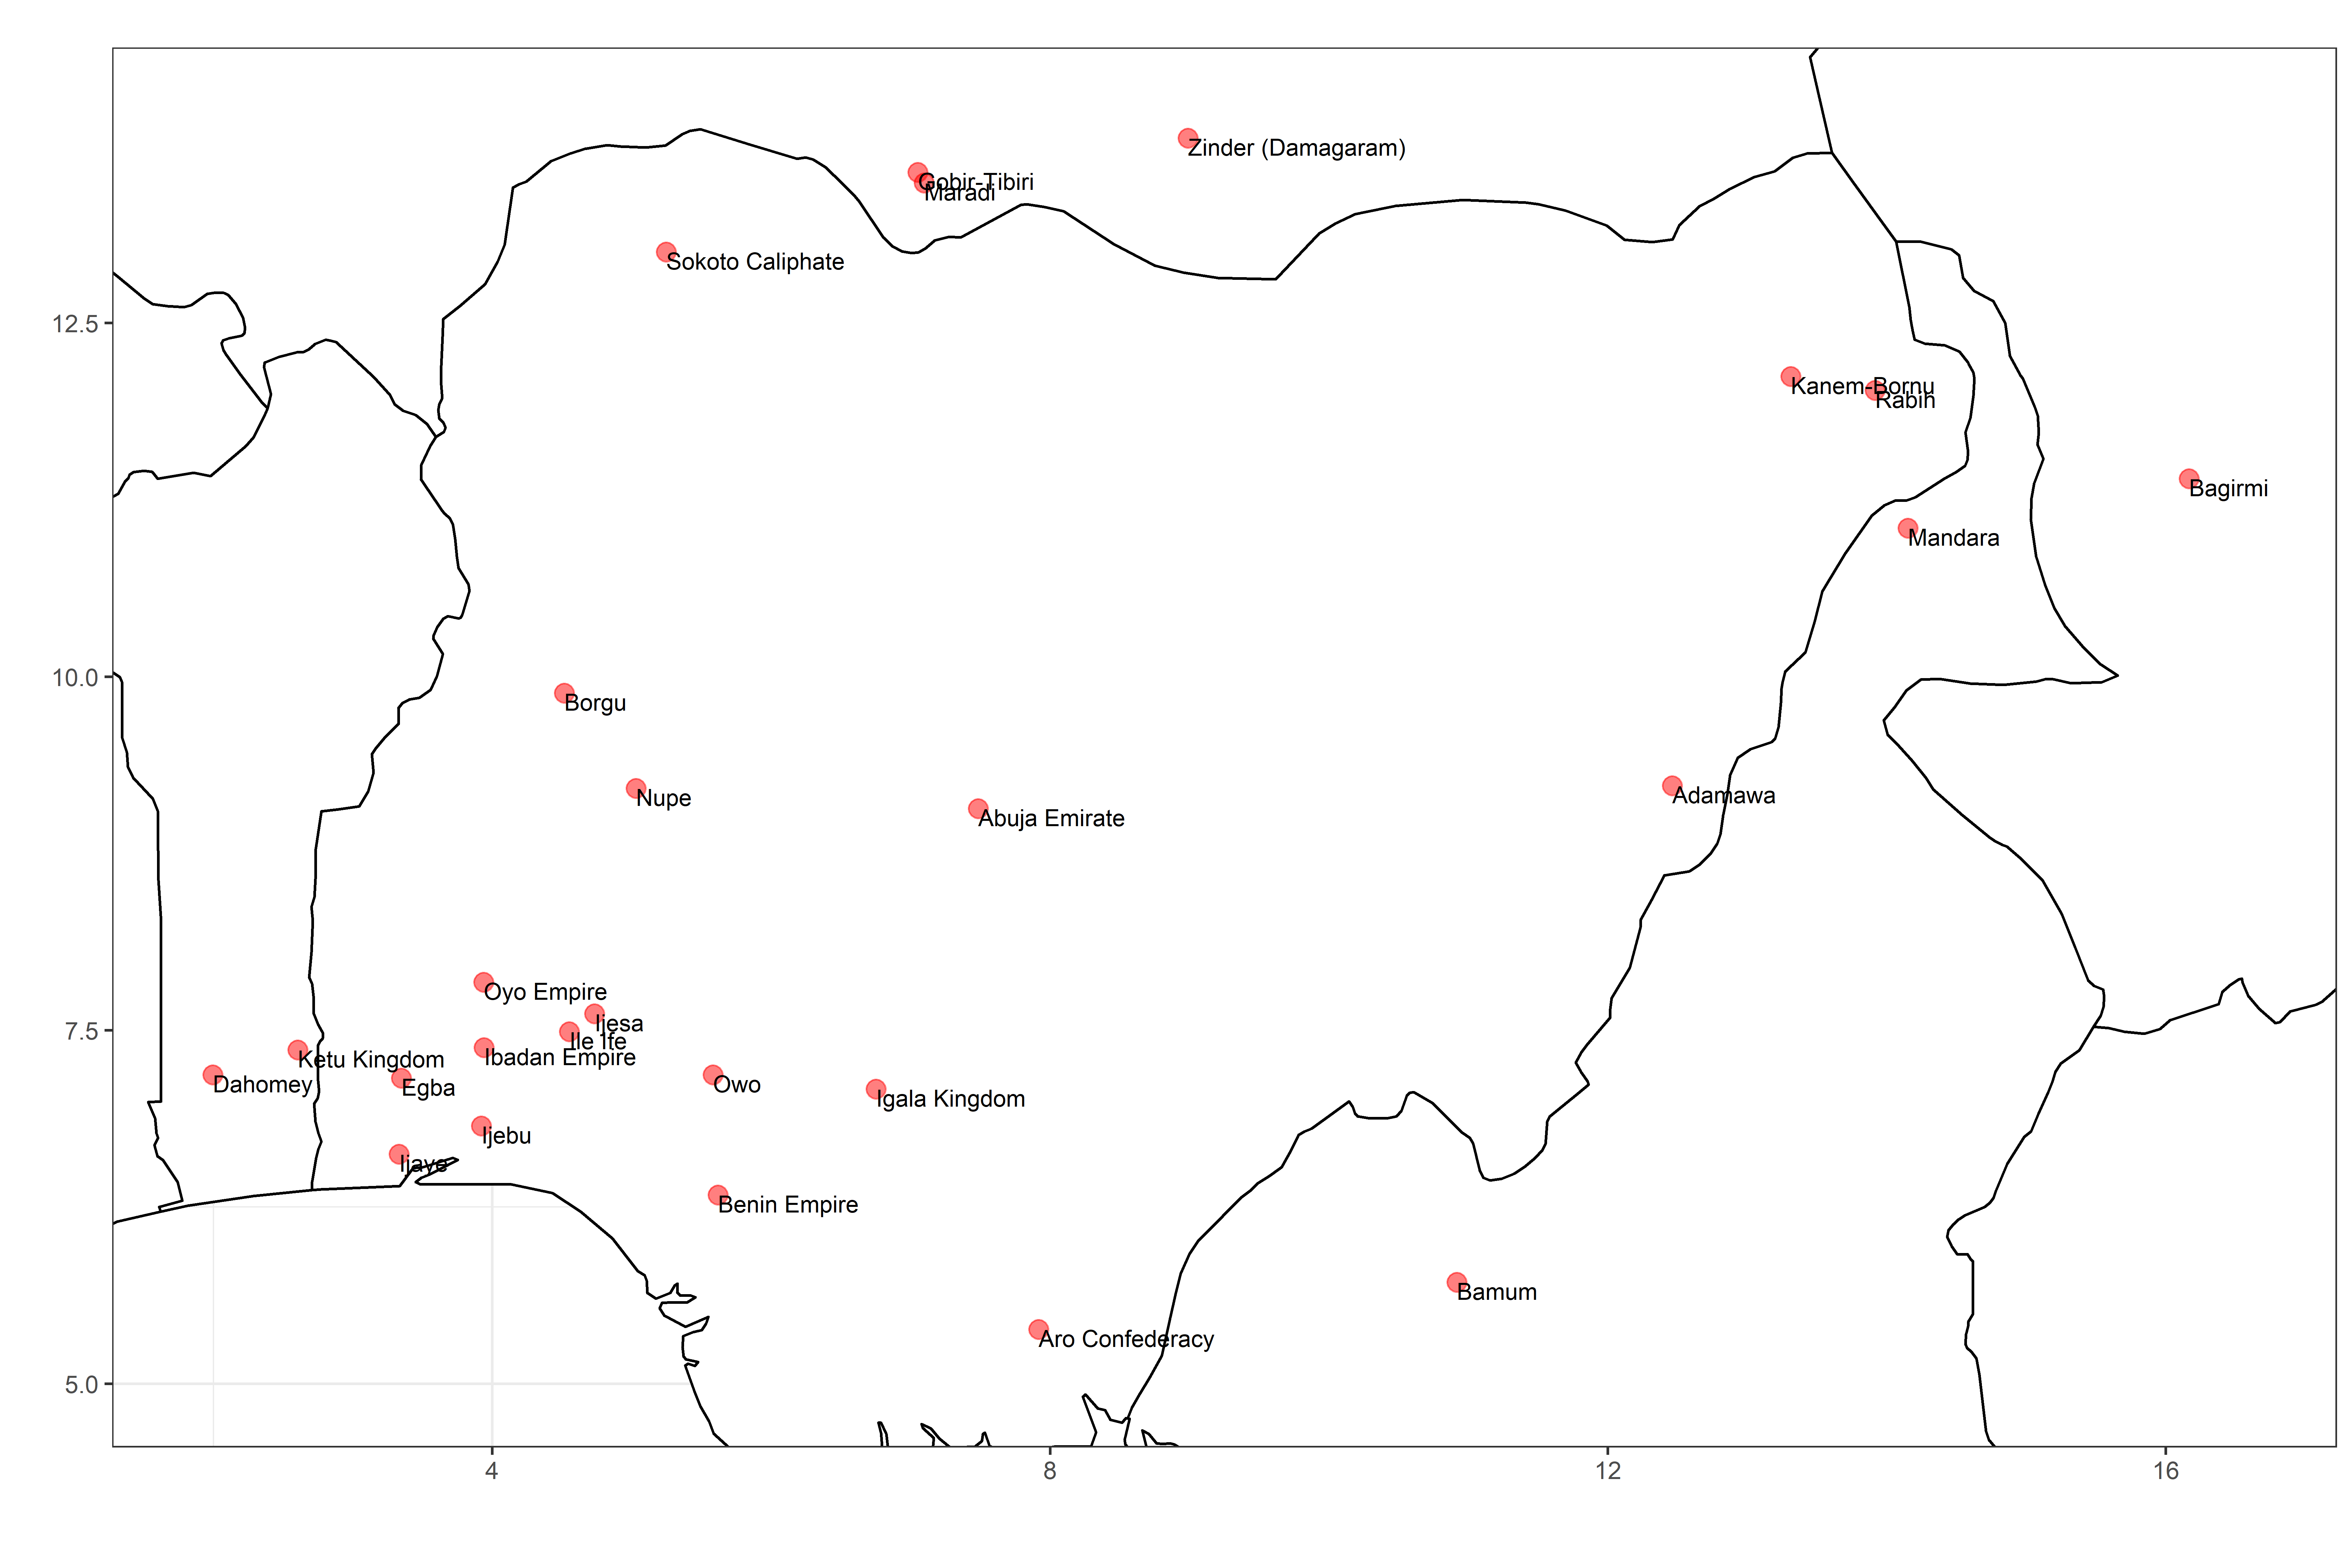
\includegraphics[width=\textwidth,
    height=\textheight, keepaspectratio]{img/isd_west_africa.png}
    \caption{Historical states in Nigeria and Surrounds, 1816-1939} \label{fig:
    westafrica} \end{figure}

Why would more HSEs in the territory of modern states lead to more internal
armed conflict? We propose four mechanisms drawn from the existing literature on
pre-colonial statehood and conflict: (1) HSEs left behind mobilization networks
useful for insurgency, (2) they left behind symbols of independent statehood
that conflict entrepreneurs can mobilize around, (3) they created the
foundations for ethnic-claim making in the post WWII period, and (4) they altered
colonial trajectories and created unfavourable conditions for democracy and
state consolidation at independence. We discuss each of these mechanisms in
turn. 

\subsection{Networks of rebellion}

Many historical states leave behind formal and informal \citep{Wig2016} social
networks that lower the costs of insurgent collective action \cite[17]{Wood2000,
Staniland2014}. For example, the Buganda Kingdom was a state entity for over 500
years before becoming a formal institution in modern Uganda through the British
system of indirect rule \citep{Tuck2005}. Buganda launched a brief and
unsuccessful armed rebellion in 1966 after a power-sharing agreement with the
Obote regime broke down \citep{Tuck2005}. In Ethiopia, the Derge regime tried to arrest the
semi-independent Sultan of Aussa (Awsa) in June 1975 \citep{Shehim1985}.
However, the Sultan was able to escape and launched an armed rebellion from
Somalia (Afar Liberation Front - ALF, \citet{Shehim1985}).  While the Sultanate
was unable to win independence, the institution continues to exist within the
current Ethiopian state \citep{Hanfare2011}. 

These are examples of HSEs surviving into the modern period as formal
institutions. Informal networks can also survive and underpin insurgency. Aceh,
for example, ruled parts of the northern tip of Sumatra in modern-day Indonesia
from the 16th to the 19th centuries. Aceh sponsored Islamic learning and became
a central node in a broad network of Islamic scholars \textit{(ulama)} in
Indonesia and Malaysia. These \textit{ulama} fought against Dutch colonialism,
even after the formal Achenese state had been destroyed. Tengku Cik di Tiro, for
example, fought in these wars and later became a symbol for Achense mobilization
against the Indonesian state. \textit{Ulama} networks survived defeat by the
Dutch and colonisation into independent Indonesia -- especially through
organizations such as the Persatuan Ulamam Seluruh Aceh (PUSA) (the All-Aceh
Assoication of Ulama)  \citep[28]{Aspinall2009} -- and formed
the core of the Darul Islam rebellion of the late 1940s and early 1950s.  The
leader of the Free Aceh Movement (GAM, formed in the 1970s), Hasan di Tiro, was the great-grandson of
Tengku Cik di Tiro -- the lauded hero of independent Achenese resistance to the
Dutch. Tiro recruited directly from these old Darul Islam networks when
launching the GAM rebellion -- networks that have their roots in the
pre-colonial Acehese state \citep[61-62]{Aspinall2009}. 


Generalising from these specific examples, historical states can leave behind
formal and informal networks that enable rebellion in the modern period. The
more historical states, the more of these legacies are left behind and --
\textit{ceteris paribus} -- the more potential foundations of rebellion there
are in the often competitive and unstable environment of post-colonial politics. 

%Numerous possible sites of rebellion might also create country-wide information
%and commitment problems that make bargaining problems with the central
%government difficult \citep{Walter2009, Cunningham2006, Paine2019}. 
 
\subsection{Symbols of sovereignty}

Historical states leave memories and collective symbols of sovereignty and
independence. These narratives of lost nationhood or stolen `homelands' can be
powerful focal points for mobilization into armed conflict in an international
system founded on the principal of national sovereignty \citep{Ahram2019,
Shelef2016}. The more prevalent these narratives are, the more common armed
conflict should be.  

There are multiple examples of armed groups using former states and empires in
this manner. The Macina Liberation Front in Mali refers to a short lived Islamic
Empire in Northern Mali that lasted for only 44 years (between 1818 and 1862,
\citep{Brown1968}). The Movement for Oneness and Jihad in West Africa (MUJWA)
`seeks to revive the “jihad” of Alhaji Umar Tell', leader of the 19th Century
Tokolor empire, and the Vanguards for the Protection of Muslims in Black Africa
(Ansaru) claims to `revive the “jihad” of Usman Dan Fodio', leader of the Sokoto
Caliphate, also a 19th Century West African state \citep{Zenn2015}. Non-Islamist
examples include the Cyranecia Liberation Army in Libya and the various
Afrikaaner resistance groups that aimed for a re-establishment of the Boer
Republics in South Africa. 

In the literature there are multiple examples of interplay between the
networks and symbols of sovereignty mechanisms. For example, The leader of the
aforementioned Free Aceh Movement (GAM) justified rebellion with recourse to
Aceh's history as a sovereign state \citep{Aspinall2009}. While in Poland, the
memory of an independent Polish state helped preserve elite networks of Polish
noblemen, and provided a model for their proto-nationalist independence movement
\citep{Wimmer2018}.

%Finally, the ULFA (United Liberation Front of Asom) was founded in an old
%palace of the Ahom Kingdom (the historical predecessor kingdom to Assam state
%in India) and draws on references to the old kingdom by, for example, claiming
%that Assam was never part of British India, referring to the treaty between the
%British and Burmese during the Assam-Burmese wars.

%\footnote{Other examples that far pre-date our data include the Islamist rebel
%group Al-Mourabitoun, whose name refers to the Almoravid dynasty who ruled
%Morocco, Western Sahara and large parts of the Iberian peninsula from the
%middle of the 11th century to the middle of the 12th century. Similarly, the
%Khmer Rouge in Cambodia also actively used the image of the Angkor Empire
%\citep{Locard2015}.} 

More historical states may therefore generate higher levels of conflict by
creating symbolic resources that dissidents can rally around and mold into
narratives of lost nationhood. These symbols -- other things being equal -- may
make it easier to initiate armed conflict against the state.  


\subsection{Ethnic power relations}

HSEs might also drive conflict by creating more `politically relevant' ethnic
groups in modern states. Existing studies tend to assume that ethnic groups
pre-date and build states \citep{Paine2019, Wig2016}, but state-building often
drives changes in ethnic identity \citep{Anderson2006, Chandra2006, Wimmer2018}.
After the First and Second World War, the increasing legitimacy of appeals to
self-determination by `national' or `people groups' rather than appeals to
effective sovereignty \citep{Clapham1996, Jackson1991}, created incentives for
collective groups to pitch political claims in ethnic or communal terms. These
ethnic claims, however, were in some cases the product of prior-state building
efforts that began before the existence of the ethnic group. 

The `Achenese', for example, are an ethnic group in the `Ethnic Power Relations'
data from 1950 \citep{Vogt2015} and the war between the Indonesian state and the
Free Aceh Movement (GAM) is coded as an ethnic conflict
\citep{Vogt2015}.\footnote{The EPR data record GAM as having ethnic claims,
recruitment and support, the highest level on all dimensions.} Aceh was a feudal-like state that portrayed itself as a pan-Islamic centre of learning before it was an ethnic group, however \citep[20]{Aspinall2009}.
The elite were mostly Malay and Arab, not people with deep indigenous roots.
\citet[46-47]{Aspinall2009} states that: `most surviving sources tell us there
was no such [Acehense] consciousness before the twentieth century'. Rather,
`Achenese' as an ethnic identity was invented by local elites to manoeuvre
within Indonesian laws that permitted `cultural' expressions and of conflict
entrepreneurs looking for foundations in international law to justify the
independence of Aceh. 

State-making also facilitated the \emph{expansion} of ethnic groups, which
influenced modern day ethnic demographics. The Lunda were a small ethnic group
in modern day Democratic Republic of Congo before the expansion of the Lunda
empire, which saw Lunda settlers spread across the DRC (especially in Katanga),
Angola and Zaire. Modern-day `Lunda' settlement patterns are therefore a product
of prior, successful, state-building. The Punjabi state of Khalistan in modern
day India and Pakistan (1799-1846) is another example of how statehood and elite
(religious) networks fused to generate ethnic tensions in the modern period, in
this case between Sikhs and the Federal Indian Government during the 1970s and
1980s \citep{Grewal1998}. Even multi-ethnic empires in the pre-colonial period
can `create' politically relevant ethnic groups in the post-colonial period. The
Sokoto caliphate was a large, Fulbe-based, but ethnically diverse Islamic empire
that conquered much of Northern Nigeria and Niger in the 1800s \citep{Law1977}.
The political `relevance' of `Hausa-Fulani and Muslim Middle Belt' in the EPR is
likely caused by the Sokoto cailphate, which (a) unified the Hausa and the
Fulani (two different ethnic groups) under the same political administration
and, (b) was the foundation for the North-South division in Nigeria because
northern Nigeria was ruled indirectly through the Sokoto caliphate while the
south was ruled more directly \citep{Paine2019}. The Sokoto caliphate was so
influential in the early politics of independent Nigeria because it
\textit{transcended} the ethnic Hausa-Fulani divide and unified the fragmented
Hausa polities under a single (albeit decentralized) Islamic administration.
These religious divisions are relevant alongside ethnic divisions in Nigeria and
the Islamic-North--Christian-South division was sharpened by the jihads of the
1800s and the establishment of the Sokoto Caliphate \citep{Reynolds1997}. 

The main upshot is that HSEs can shape post-colonial ethnic relations by
creating, unifying and expanding ethnic groups into conglomerates that became
`politically relevant' in an international system that privileged `national'
claims (i.e people-group claims) over claims based purely in prior state rule.
Countries with more historical states may be at a higher risk of conflict
because those countries have a higher number of claims-making ethnic groups in
the post-colonial period. To the extent that more ethnic groups or ethnic groups
with a history of statehood create bargaining problems and highly competitive
political environments characterised by ethnic exclusion and favoritism
\citep{Paine2019, Roessler2016, Cederman2013}, this should also increase the
number of armed conflicts. We do not attempt to untie the knot of ethnicity and
statehood here, but existing research establishes a link from historical states
to modern-day civil conflict that plausibly runs through a higher number of claims
making ethnic groups that are themselves the product of state-building efforts.

%\footnote{This argument does not contradict studies of historical statehood and
%modern ethnic groups, although it it does point to a potentially confounding
%variable - prior statehood.} 

\subsection{Colonialism, Democracy and Weak Statehood}

Historical states often resisted European colonialism and where they were
colonised, were ruled indirectly rather than directly \citep{Gerring2011,
Hariri2012, Englebert2000}. Areas with stronger `indigenous' statehood were also
more successful at resisting European cultural and religious influences,
especially Protestant missionaries \citep{Woodberry2012}. Although the
connection is debated, direct colonial rule and the influence of Protestant
missionaries may have created some foundations for democratic rule in the
post-colonial period \citep{Woodberry2012, Hariri2012} and democracies are less
likely to experience civil conflicts than semi-democracies or autocracies
\citep{Hegre2006}.

In addition, indirect rule preserved some of the power and influence of
historical states through the colonial period, placing them in a stronger
position to place demands on colonial regimes during the decolonization process
and the leaders of newly independent states. Where there were many HSEs, this
can create a `strong society, weak state' dynamic where the central government
struggled to rule parts of its territory where HSEs survived, creating areas of
weak state control which, as \citet{Fearon2003} and \citet{Lewis2017} argue, can
facilitate insurgency by reducing the likelihood of state detection and defeat
in the initial stages. \citet{Herbst2014} argues, for example, that colonial
regimes in Africa concentrated their rule in coastal capital cities, leaving
existing institutions largely intact in the hinterland. At independence, African
leaders inherited weak states with little `infrastructure' of rule outside of
the capital, faced strong challengers and high costs to expand the state. This
dynamic was replicated in South Asia and South-east Asia \citep{Migdal1988} and \citet{Mazzuca2021} observes a similar dynamic whereby conditions at the moment of state formation -- especially strong regional powers -- help explain state weakness in South and Central America.
Recent research suggests that \textit{expanding} state presence can drive the
onset of new internal armed conflicts \citep{Ying2020}, and as modern states
move into areas previously ruled by HSEs, armed conflicts can become more
likely. Higher numbers of HSEs may therefore generate more armed conflict in
post-colonial period by altering the trajectory of colonial rule and creating
conditions where weak, non-democratic states emerged after independence that
faced strong internal challengers. 

\bigskip

Figure \ref{Fig: CausalDiagram} outlines the main mechanisms that link HSEs to
conflict: (1) Networks of Rebellion, (2) Symbols of Sovereignty, (3) Ethnic
Power Relations and, (4) Colonialism, Democracy and Weak Statehood. Additional cases exhibiting links between HSEs and modern conflicts can be found in the appendix.

    \begin{figure}[!htb] \hspace{-0,5cm} 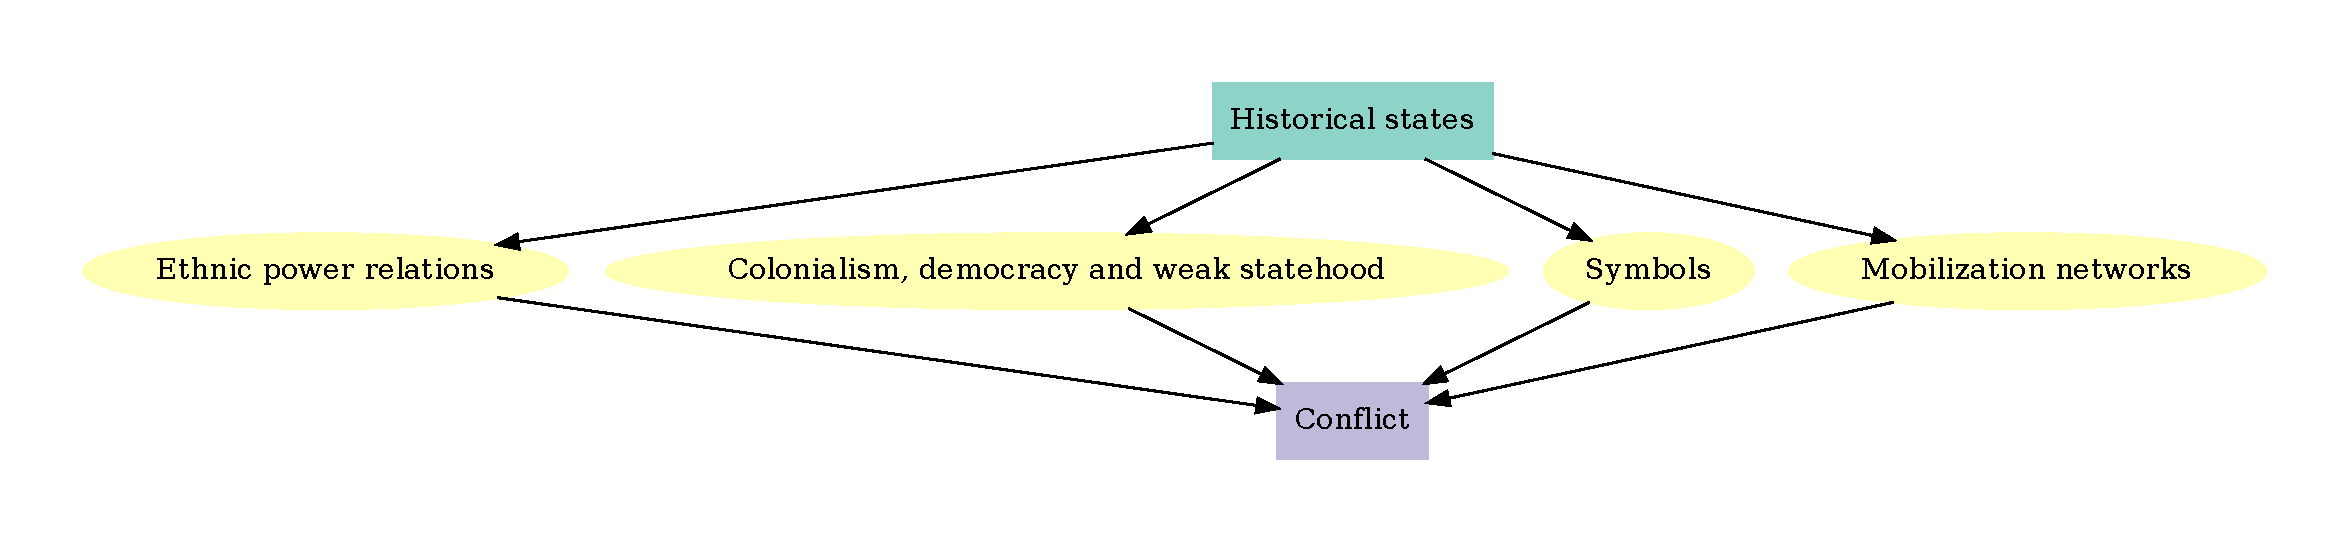
\includegraphics[width=\textwidth,
    height=\textheight, keepaspectratio]{img/graf.pdf} \caption{Causal diagram}
    \label{Fig: CausalDiagram} \end{figure}

Hypothesis 1, outlines the bservable implications of our arguments. 

\bigskip

\hangindent = 3.5em \textit{H\textsubscript{1}: More historical states in the
territory of a modern state increase number of internal armed conflicts}

\subsection{Conditional effects}

Our argument is general and probabilistic applying to the post WWII period. It should not be taken to mean that all HSEs are conflict inducing or that all conflicts involve HSEs. Studies show that in some instances, historical states can be advantageous to state-building by providing pre-fabricated governance structures that the centre can draw upon to deliver public goods and peace \citep{Ziblatt2008}. Historical states can be assets for state-building when the expanding centre and the historical states have high ``infrastructural capacity'', meaning a high capacity for taxation, providing public order and delivering public goods. In these circumstances, bargaining occurs between strong and credible actors capable of delivering on agreements \citep{Ziblatt2008, Wig2016}. These circumstances do not characterise the state-building challenges of most states in the post-WWII period, especially post-colonial states. First, the centres often inherited weak and geographically limited infrastructural capacity at independence \citep{Herbst2014, Migdal1988}. Second, most historical states in our sample were relatively weak and decentralized, especially in Africa, Southeast Asia and South Asia \citep{Herbst2014, Scott2009}. We also suspect that some of the paradigmatic examples of peaceful state-HSE integration are also situations with few HSEs, as characterises modern day Ghana, or Benin. The typical conditions under which modern and historical states combine for effective state-building, therefore, do not characterise the situation of most states in the post-WWII and we, therefore, expect a general \textit{negative} effect of more HSEs on peace as they provided the resources for collective action in a situation where effective bargaining is difficult. 

We do, however, make two conditional arguments based on the discussion above. First, we expect that HSEs are less dangerous when they are located closer to the modern capital. The \textit{process} of state consolidation often causes conflict between the centre and peripheral regions \citep{Ying2020}. As the costs of governance increase with distance from the centre in many modern, especially post-colonial, states \citep{Herbst2014}, HSEs located closer to the modern-day capital should be easier for the centre to incorporate peacefully. These may also be HSEs with pre-existing connections to the centre through trade and transport infrastructure. Historical states located close to the capital also sometimes inherit the state (such as in Egypt, Thailand, Sweden, or China), entailing a smooth transition between the historical and modern state. In contrast, HSEs located far from the capital are more likely to be disconnected from the centre and far more costly for the centre to incorporate, either through force or negotiation. 

Second, modern states with more economic resources may be able to avoid conflict by providing economic transfers to regions with HSEs, or alternatively, modern states with higher levels of development may contain HSEs with a higher pre-existing level of development, or interconnectedness, making them easier to incorporate. Italy, for example, may have been able to avoid conflict in the post-WWII period, despite multiple HSEs, due it's higher capacity to incorporate former states. Sardinia and Sicily (both HSEs), for example, have had active secessionist movements, but these never escalated to high levels of armed conflict \citep{Griffiths2016}. Germany's federal institutions are (in general) the product of effective negotiation between a developed centre (Prussia) and numerous, relatively developed regional kingdoms \citep{Ziblatt2008}.  More developed artificial states should therefore have a larger carrying capacity for historical states and be better able to solve bargaining problems peacefully.  

These conditional arguments imply two hypotheses:

\hangindent = 3.5em
\textit{H\textsubscript{2}: The number of historical states in the
territory of a modern state has a stronger positive impact on internal armed conflicts when those states are located further from the modern capital}

\bigskip

\hangindent = 3.5em
\textit{H\textsubscript{3}: The number of historical states in the
territory of a modern state has a stronger positive effect on the probability of civil war in less developed states}

\bigskip

 
\section{Research design}

\subsection{Dependent variables}

The unit of analysis is a country, observed over the 1946-2019 period. Our
dependent variable is the conflict onset rate over the 1946-2019 period, sourced from the UCDP/PRIO Armed Conflict
Dataset \citep{Pettersson2020}. A new onset is recorded when a state experiences
a new internal or internationalized internal civil conflict after a period of
two or more years of no conflict. The dependent variable is divided by the number of active state years to adjust for exposure time. Onsets represent
attempts at armed rebellion successful enough to cross the UCDP death-threshold
of 25 battle related deaths in a year \citep{Tollefsen2012,
Lewis2017}.  Our mechanisms
describe conditions conducive to the launching of rebellion rather than the
number of rebel groups \citep{Fjelde2009}, conflict duration
\citep{Cunningham2006} or termination \citep{Walter2004} that are explained by
additional processes such as splintering, bargaining failures with multiple
rebel groups and peacekeeping.\footnote{Using our main models, modern states with more HSEs also experience a higher rate of armed conflict incidence ($p<0.05$) and incidence of years with more than 1000 deaths ($p<0.10$).} 
The main results reported below are robust to several variations on the dependent variable, including using the logged number of onsets, the rate of logged onsets and the raw count of onsets using both negative binomial models for over-dispersed count data and OLS regressions. 

\subsection{Independent variables}
    
The independent variable is a count of the number of HSEs that existed between
1816 and 1939 in the territory of a modern state (i.e a state that existed
between 1946 and 2019). These data are sourced from version two of the
International Systems Dataset (ISD). \cite{Butcher2020}
require that polities have more than 10,000 people, autonomy over a specific
territory and uncontested or recognized external sovereignty in order to qualify
as a state. These criteria are more inclusive
than the COW State System Membership List \citep{Sarkees2010} but more
restrictive than the Murdoch map (1967) that also includes stateless ethnic
groups. 

To code the `destination' state of HSEs we used the latitude and longitude
coordinates in the ISD for approximate locations of HSE capital cities. We
overlay these capitals on modern borders and count how many capitals fall into
those borders. HSEs often ended up in multiple territories -- parts of the
Sokoto empire, for example, are in modern-day Nigeria, Niger, and Cameroon -- and
we coded up to ten additional destination states based on locations specified in
the World Statesmen database of traditional states
(\url{https://www.worldstatesmen.org}) and our own searches of secondary
sources. Historical states in the ISD do not necessarily overlap in time. Some
historical states can disappear, while others can come into being during the
sample period, within a given territory. Because this measure does not vary
across time, we use cross-sectional analyses to avoid artificially inflating the number of observations.  Figure \ref{Fig:
ISDstates} shows how many historical states (i.e states that existed at some
point between 1816 and 1939) are recorded within the boundaries of modern
states. We also run models below counting only the number of historical state
\textit{capitals} falling within the borders of a modern state, with very
similar results. 
    
The ISD has a number of advantages. The first is global coverage. Existing
studies have primarily analysed Africa, or Sub-Saharan Africa, while there were
dense states systems in South Asia, Southeast and East Asia, and South America
that are excluded by these analyses. Even within studies of pre-colonial Africa, many
state entities are not included. For example, \citet{Besley2014} use data for
19 historical kingdoms in Africa over the 1400-1700 period to assess the impact
of historical conflict, while our sample includes 109 states on the African continent
that were independent at some point over the 1816-1939 period.

    
Second, the ISD includes states without selecting on ethnicity.
States that were ethnically based are included (such as Buganda), along with
multi-ethnic empires such as the Sokoto Caliphate and states that were not
ethnic such the Rajput states of India, which were based
more upon a shared warrior `class' than ethnicity \citep[12]{Ramusack2004}. This
provides a more accurate picture of statehood in the 19th century, even within
Africa. For example, \citet{Paine2019}'s recent study of pre-colonial
ethnic-states and post-colonial conflict identifies just one state in Ethiopia,
while the ISD identifies eleven, some of which were highly centralized, such as
the Shoa or Jimma kingdoms \citep{Lewis2001}. Thus, what \citet{Paine2019}
identifies as a country with one ethnic-state that is otherwise `stateless', is,
according to a different dataset, a country with multiple historical states. By
avoiding the assumption that states are ethnic states we also avoid projecting
modern ethnic identities back onto pre-colonial polities that were not
ethnically based or only marginally so.

    \begin{figure}[!htb] \hspace{-0,5cm} 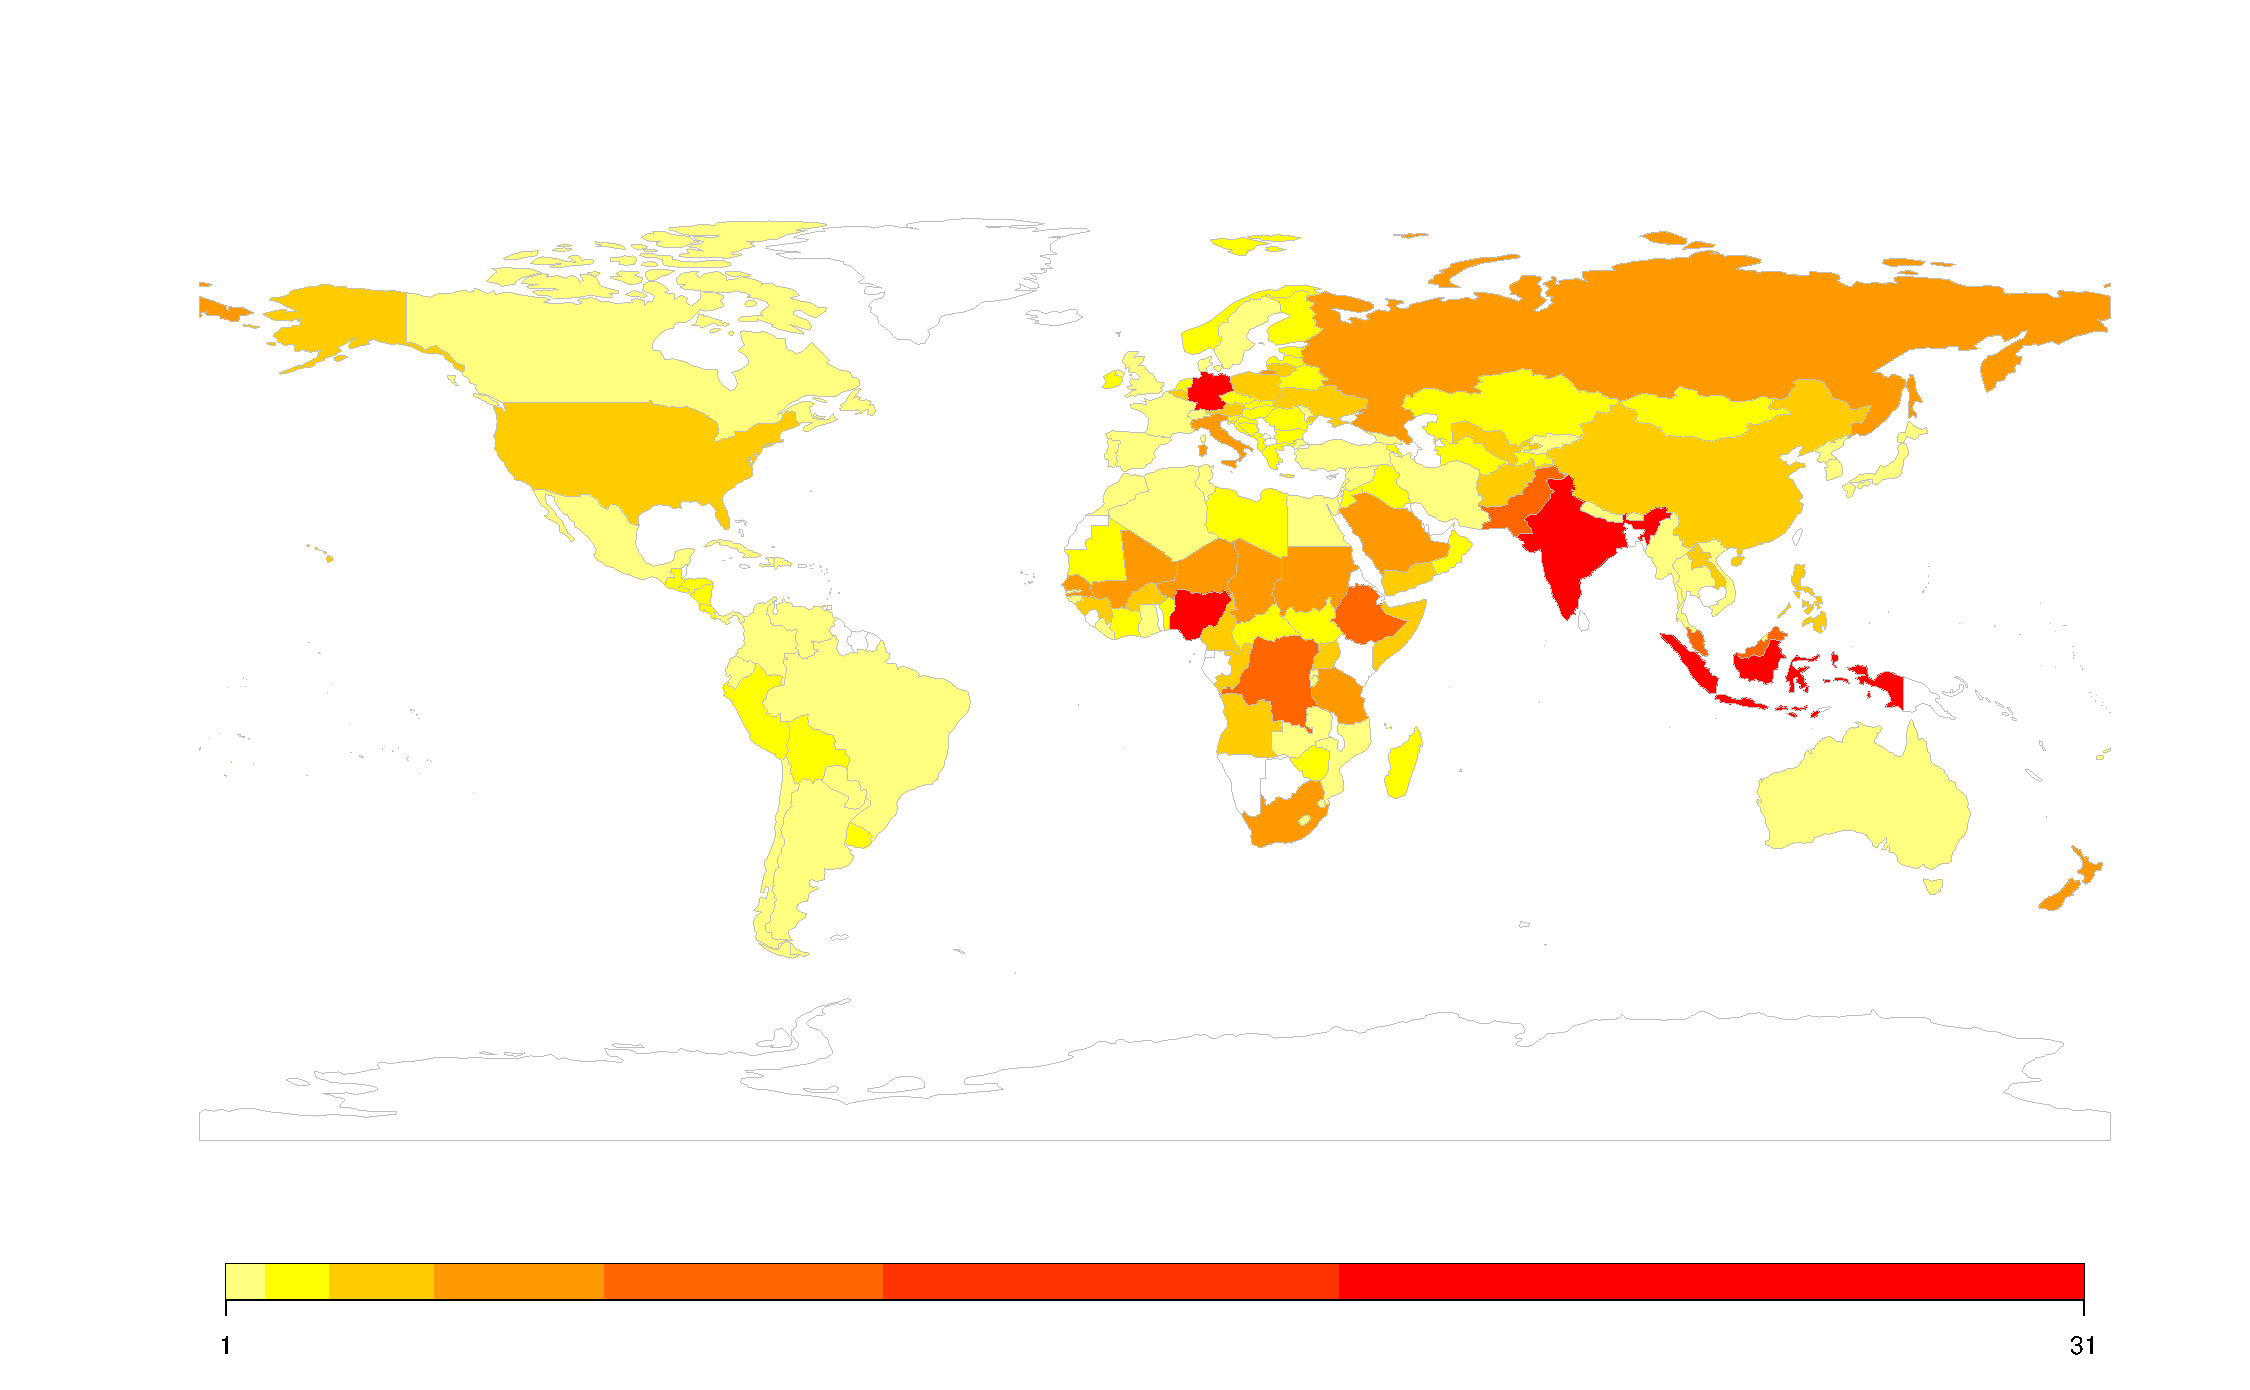
\includegraphics[width=\textwidth,
    height=\textheight, keepaspectratio]{img/statesplot.pdf} \caption{Number of
    historical state entities per country} \label{Fig: ISDstates} \end{figure}
    
The main drawbacks are that the ISD start in 1816, and only geocode capital
cities or state centres. Eighteen-sixteen is an arbitrary starting point,
marking the Congress of Vienna and the aftermath of the Napoleonic wars, that attributes some states with no HSEs because they were colonised before 1816
(e.g Bangladesh) and elides historical states that existed in the 1700s and
earlier, some of which may have powerful legacies (especially in Europe, India
and Myanmar). However, the 1816-1939 period is also a critical period, and
arguably more important than earlier periods of historical statehood for
understanding modern conflict dynamics because these states existed on the eve
of the international system freezing into its current territorial divisions through
colonialism, followed by the explosive rise of norms emphasising
self-determination and fixed territorial sovereignty \citep{Branch2013, Ahram2019,
Paine2019}. Some states, such as France, Sweden, Thailand or China entered this
international system having already incorporated historical states through
processes of vassalage, warfare, territorial expansion and centralization by the
end of the 19th century. Other states fared very differently. Nigeria, for
example, did not exist as a state before 1960 and the territory of modern-day
Nigeria is host to numerous historical states that existed between 1816 and
colonialism, many of which survived through colonialism (and because of
colonialism) and indirect forms of rule. These were all potential challengers to
the post-colonial Nigerian state. \citet{Mazzuca2021} shows that conditions at the moment of \textit{state formation} can have lasting impacts on the trajectory of \textit{state consolidation}. If we were to go further back in time, we
would surely find more states,\footnote{Burma, for example, conquered many of
the independent Burmese states in the late 1700s and has seen widespread armed
conflict (41 onsets in our data).} but measuring independent
states that existed between 1816 and 1939 captures the main historical states
that presented the greatest potential conflict risk in the modern period.\footnote{Some resources such as GeaCron map statehood globally back into the 1600s and 1700s, but underestimate the number of states and
conflate non-state entities with states. For example, GeaCron
identifies just 15 states in Africa in 1840 where the ISD identifies 92 and
includes the ``Hausa'' in Nigeria, which was not a state but a collection of independent city-states} 

\subsection{Controls}

Our identification strategy rests upon conditioning on observable factors
\citep{Morgan2015}, making the question of what causes higher or lower numbers
of historical states in the territory of a modern state critical. Before
discussing control variables, the number of historical states is likely
exogenous to some factors that may cause armed conflict. State formation is not
random \citep{Tilly1990, Osafo-Kwaako2013, Bates2008}, but the \emph{number} of
states encompassed by modern boundaries depends upon the boundary-drawing
process. 
Competition between European powers generated colonial boundaries that were
quasi-random in relation to local conditions \citep{Clapham1996, Branch2013,
McCauley2015}. \citet[3]{McCauley2015} suggest that up to 80\% of the borders in
Africa follow `meridians, parallels or other rectilinear or curved lines'. The
`Scramble for Africa' is infamous for paying little to no attention to local
conditions when demarcating colonial spheres which eventually became the
foundations of modern state boundaries \citep[32-34]{Michalopoulos2018}. 
Moreover, some of the risks associated with assuming quasi-random border
allocation highlighted by \citet{McCauley2015} -- especially cluster
randomization and open treatments -- do not apply in our case because we are not
studying individuals and HSEs cannot move after 1939. Therefore our independent
variable is partially assigned by a process that is likely to be independent of
factors that cause modern conflict. At the very least, our results are not
likely to be explained by reverse-causality concerns in some samples, especially
the African sample.  
    
Nonetheless, borders are not exogenous in an experimental sense. Even in Africa
some borders were drawn in relation to historical states -- the Sokoto caliphate
and the northern Nigerian borders are an oft-cited example \citep{McCauley2015}
-- and borders in Southeast Asia, South Asia, Europe, and Central Asia may have
been drawn more in response to local conditions given the longer colonial
experience in these areas or due to longer term processes of war and absorption.
Moreover, the number of historical states will also be a function of how
conducive the conditions within modern borders are to state-building, no matter
how random the assignment of borders are. Our main models include a parsimonious
set of controls and we show results with an extended set of controls.

Population density is closely related to state-building \citep{Herbst2014} and
the `great reversal' entails that countries with favourable conditions for
state-building had lower levels of economic growth in the modern period
\citep{Acemoglu2001}, making them more vulnerable to armed conflict
\citep{Fearon2003a}. We control for estimated population density in 1500 from
\citet{Dincecco2019}.\footnote{Unless otherwise states, our control variables
come from replication data in \citet{Dincecco2019}}  Larger countries have more
space for previous state entities and may be more difficult for states to
govern. A control for land area in 1000s $km^2$ was included. Countries that
were colonized by Europeans may also contain more historical states compared to
un-colonized countries because Europeans often drew borders without respect to
historical states as opposed to more indigenous processes of state building,
absorption and separation that may leave fewer historical states behind
\citep{Tilly1990}. The link between European colonialism and civil conflicts is less
clear, however \citep{Hegre2001}. A control for whether the state was a former
European colony from the Correlates of War Colonial Contiguity data was included
\citep{CorrelatesofWarProject2016}. A control for historical conflict from
\citet{Dincecco2019} was included, as conflict can drive state-building
(although this is contested \citep{Osafo-Kwaako2013}) and may be related to
armed conflict through other channels such as lower trust \citep{Besley2014} or
lower levels of development \citep{Englebert2002}. Additional tests exploring historical conflict as an alternative explanation can be found in the appendix and suggest that historical conflict does not confound the main results. The timing of the neolithic
revolution has been found to drive state-building and conflict \citep{Paine2019}
and we control for this with the log of years since the neolithic revolution. We
also control for the log absolute latitude and for slave exports as slavery may
have inhibited or promoted state-building while undermining trust that may have
led to conflict \citep{Nunn2008}.

The average number of politically relevant ethnic groups in the Ethnic Power
Relations data (EPR; \citet{Vogt2015}) over the 1945-2017 period was included.
This is a post treatment control that biases against the main hypothesis. Some
ethnic groups may have pre-dated states and caused conflict through other
channels than state-building, while some ethnic groups were created by states
and may be a modern phenomena. By controlling for both, we remove the causal
effects of more EPR ethnic groups on conflict that are independent of historical
statehood and the effects that run though prior statehood, biasing our estimates
down. This is a conservative approach but reduces the risk that our results
reflect a simple `more ethnic groups = more states = more conflict' story, or
whether our measure of historical statehood is simply picking up the measurement
error in estimates of ethnic diversity, where it is also difficult to
disentangle the relationship between ethnicity and statehood. We also include
the ethnic fractionalization index, which measures the extent to which ethnic
demographics are dispersed across many groups or concentrated in a single group.
By including both of these popular measures of ethnic diversity, we can be more
confident that our results do not reflect only pre-existing ethnic conditions.
Finally all models include region fixed effects for Sub-Saharan Africa, the
Middle East and North Africa, Eastern Europe and Central Asia, Latin America and
the Caribbean, Western Europe and North America and Asia and the Pacific. These
controls parse out any region-specific factors that drive state-building and
conflict.  

These controls are the baseline controls included in all the main models. We
also ran models with additional controls for geographic factors, specifically
the country's suitability for agriculture, the extent of rugged terrain and
whether it was an island or landlocked. Again, these controls come from
\citet{Dincecco2019}. 

\subsection{Modelling strategy}

We follow \citet{Besley2014} and use Ordinary Least Squares (OLS) regressions.
The first two models use the civil conflict onset rate over the 1946-2019
period as the dependent variable, with the main and geography
controls. Models with the dependent variable disaggregated into conflicts over
government, conflicts over territory and then the onset rate in the
1946-1988, 1989-2000 and 2001-2019 periods are then shown. Results in regional
and theoretically relevant subsamples follow. We then re-test our hypothesis
against four similar, but conceptually distinct, independent variables: (1) the
number of ethnic groups with centralized states, from \citet{Wig2016}, (2) the
number of ethnic groups with pre-colonial states (PCS) and `stateless' ethnic
groups in PCS states from \citet{Paine2019}, (3) state antiquity from
\citet{Bockstette2012} and, (4) the fractal index from \citet{Alesina2011}. The
last section unpacks the mechanisms using mediation analysis and explores conditional effects, discussed in more
detail below. 

\subsection{Mediated and conditional effects}

The main models aim to identify the general association between more historical
state entities and the number of conflict onsets. We also use mediation analysis
to explore the channels through which historical statehood might affect conflict
\citep{Imai2011}. The mediation models use the baseline control variables.
Testing the networks and symbolism argument is difficult because the legacies of
past states take many forms -- ethnic networks, religious networks, states in
federal systems, symbolic cultural or political roles -- and there are no cross
national measures of these concepts (outside of ethnicity) that we are aware of.
However, we can test the ethnicity and weak-statehood and colonialism mechanisms
with cross-national data on ethnic groups, indicators of state development and
patterns of colonial experience. 

To test the colonialism argument we use colonial duration, similar to
\citet{Hariri2012} and the estimated percentage of people evangelised by
Protestants in 1923 from \citet{Woodberry2012}. Colonial duration and
`conversionary protestants' have been shown to positively impact civil society
and democracy in the post World War 2 period. 

To test the ethnicity mechanism, we use the average number of politically
relevant EPR groups across the 1945-2017 period and the average number of
politically excluded EPR groups over the same period as mediators. Data come
from the EPR project \citep{Vogt2015}. These mediators capture ethnic groups
that pre-dated states and ethnic groups that were created by states (such as
Aceh). We cannot separate these two channels but the mediation analyses provide
an indicator of whether any HSE-conflict link is primarily explained by the
creation or survival of modern-day ethnic groups. 

Finally, to test the state-weakness argument we use log GDP per capita in 2000
from \citet{Acemoglu2001} and relative tax capacity \citep{Hendrix2010} as
mediators. A statistically significant mediated impact would suggest that HSEs resulted in weak state capacity and higher levels of armed conflict, but it could reflect
the impact of earlier conflicts on GDP per capita. The estimate is therefore
biased towards finding a mediated relationship. No significant association,
however, would constitute stronger evidence against this as a causal channel. 

Hypotheses two and three imply conditional effects. To test $H_2$ (HSEs have a stronger effect when located far from the capital), we create a variable capturing the average distance between the first modern capital and the capitals/centres of HSEs and interact this variable with the number of HSEs. To test $H_3$ (HSEs have a stronger effect in less developed states), we interact the number of HSEs with the
first non-missing observation of GDP per capita after 1946 from The Madison
Project to assess whether HSEs are primarily associated with conflict in states
that lack the economic capabilities or preexisting state capacity to absorb
them.   

\section{Results}

\subsection{General associations between HSEs and armed conflict}

Figures \ref{Fig: Main_Scatter} and \ref{Fig: Onset_rates} show bivariate
associations between HSE prevalence and modern conflict onset rates. Countries
with more HSEs are associated with higher armed conflict onset rates. From
Figure \ref{Fig: Onset_rates}, a state with no HSEs (e.g Malawi) experienced
conflict onsets in 2.5\% of state years, which doubles to 5.1\% for one HSE,
before dropping to 2.5\% for states with two HSEs. \footnote{Myanmar, which
unified in the late 1700s, largely accounts for the increase at one HSE. States
with one HSE have an average onset rate of 4\% if Myanmar is dropped} Onset
rates then steadily climb until states with more than 10 HSEs expect onsets in
19\% of country years. The increase is more pronounced for territorial
conflicts.

\begin{figure}[!htb]
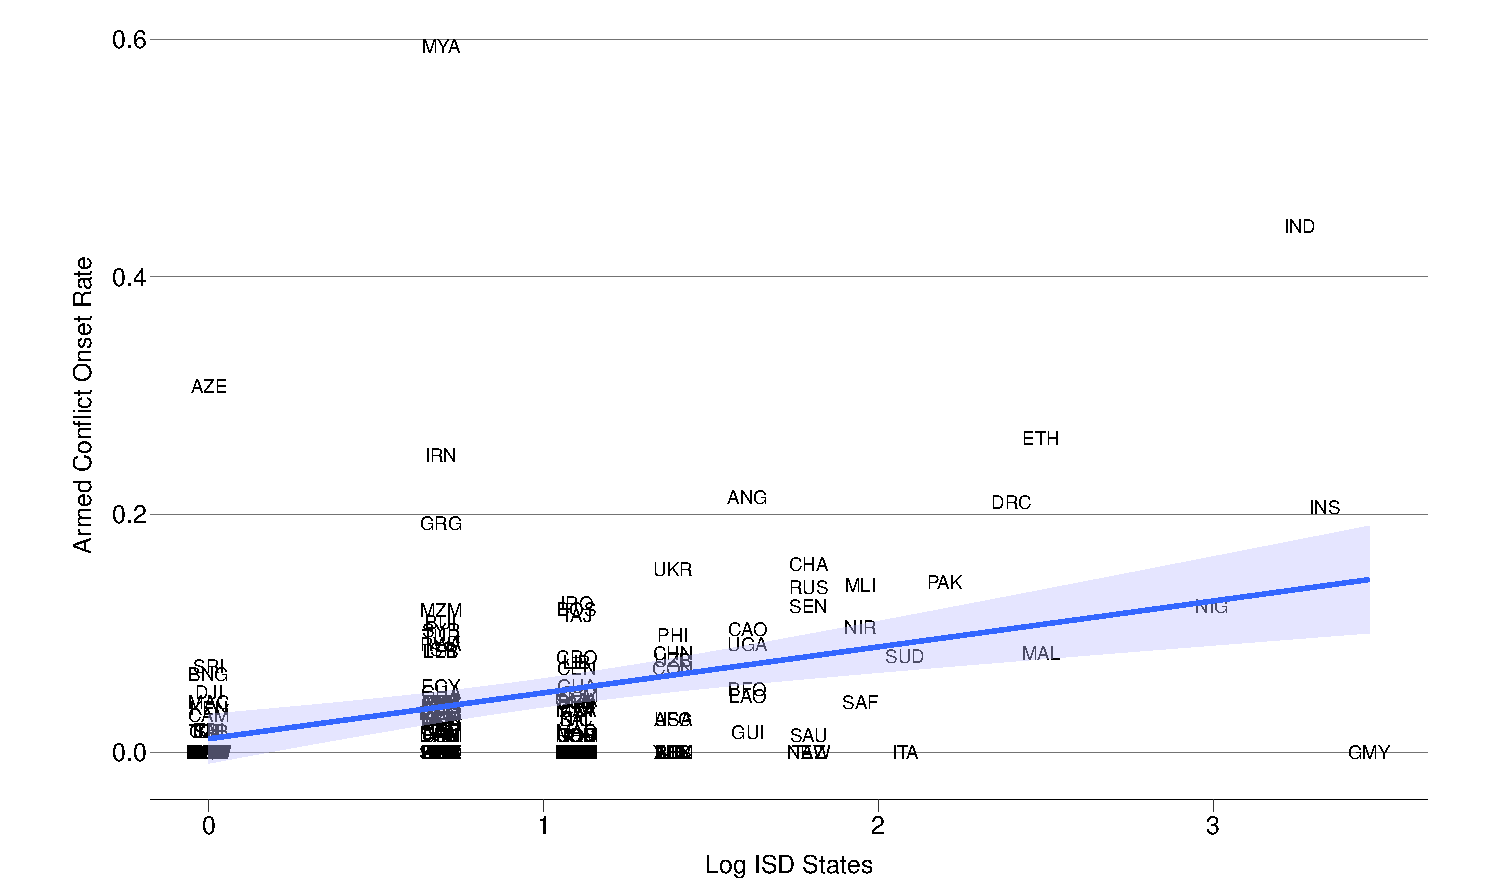
\includegraphics[width=\textwidth,keepaspectratio]{img/hse_scatterplot.pdf}
\caption{HSEs and Armed Conflict, Bivariate Association} \label{Fig: Main_Scatter}
\end{figure}


\begin{figure}htb]
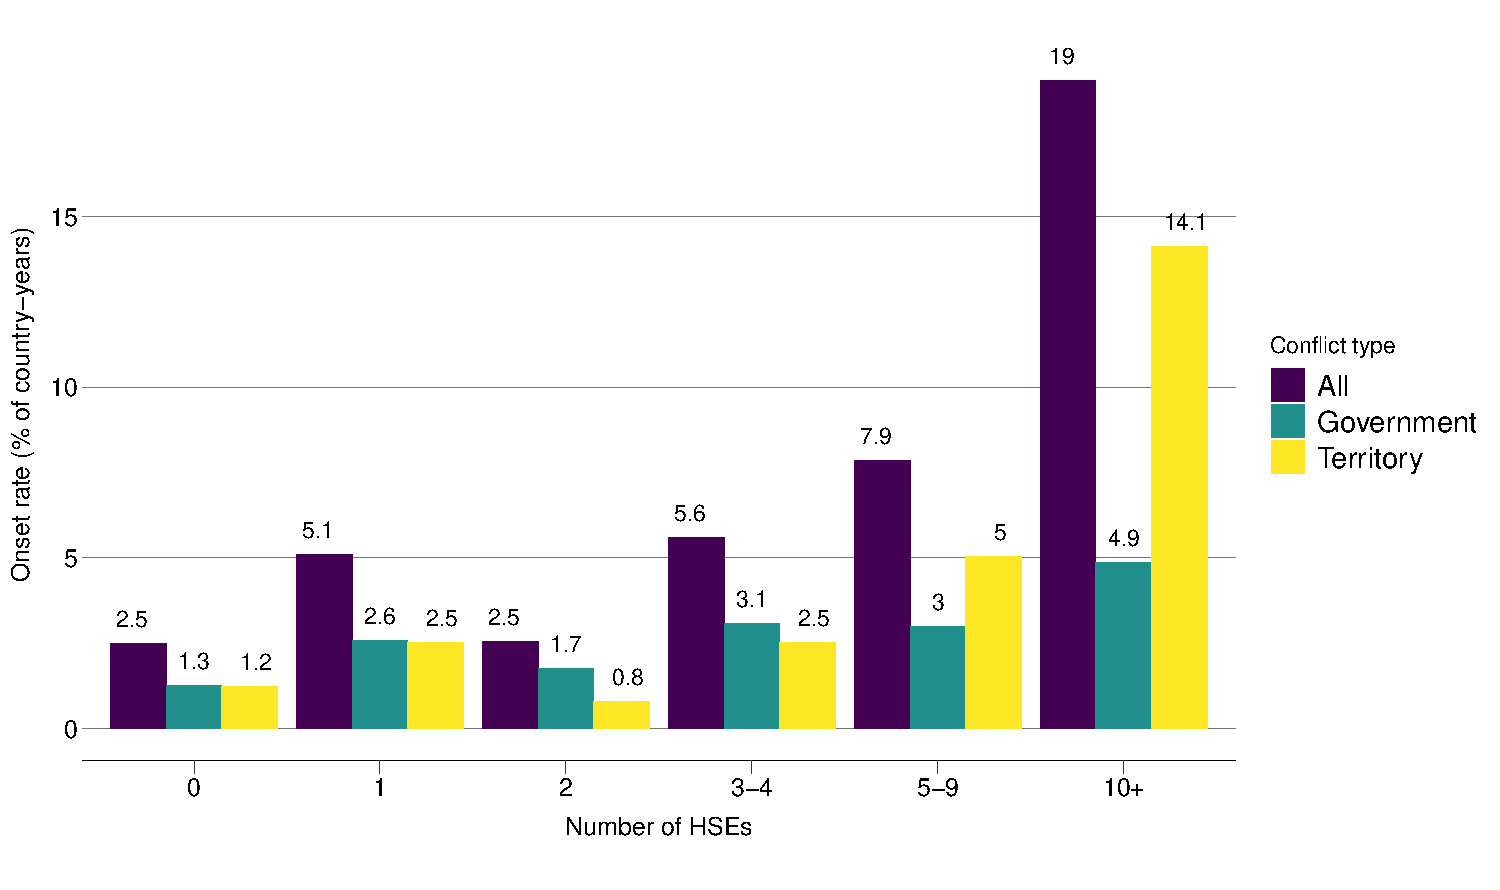
\includegraphics[width=\textwidth,keepaspectratio]{img/hse_onset_rates.pdf}
\caption{Onset rates across HSEs and conflict types} \label{Fig: Onset_rates}
\end{figure}

Figure \ref{Fig: Main_Margins} shows results using the main dependent variable
(internal armed conflict onsets) and our main robustness tests. The regression
tables can be found in the Appendix. There is a consistent positive impact of
HSEs on the number of internal armed conflict onsets. The association is
significant across both batteries of controls and is therefore likely to be
independent of important alternative explanations: that HSEs are symptomatic of
many ethnic groups in the modern period or that these are countries with an
underlying propensity to state-building and conflict. We ran a sensitivity
analysis using the \texttt{sensemakr} package in \texttt{R}, which can be found
in the Appendix. A confounder that would render the main results insignificant
would have to explain about 8\% of the variance in the number of ISD states
\textit{and} the conflict onset rate. For comparison, not even confounders
explaining three times the variance as the average number of EPR groups or the
measure of historical conflict would render the results insignificant at the
0.05 level.  Other things being equal, moving from the number of HSEs in Tunisia
(1) to the number in Nigeria (19) is associated with an onset rate that is 0.08
points higher, or about one additional armed conflict onset every twelve years.
Although the model is not specifically set up to estimate the impact of ethnic
group identities on conflict, we would need to add more than 10 politically
relevant ethnic groups to generate the same impact on conflict onset (on average
there were 6 politically relevant EPR groups in Nigeria over the 1946-2017
period and 0 in Tunisia). Thus, the main association is of a similar magnitude
to the association with politically relevant ethnicity. 

The positive association between HSEs and armed conflict applies to conflicts
over territory and to a lesser (although still statistically significant)
extent, armed conflicts over government. The results are also fairly stable over
time periods. Using the baseline model, more HSEs increase the number of
expected conflicts during the 1946-1988 period, the 1989-2000 period and the
2001-2019 period. In general these results
indicate a resilient association across conflict issues and time
periods. 


\begin{figure}[!htb]
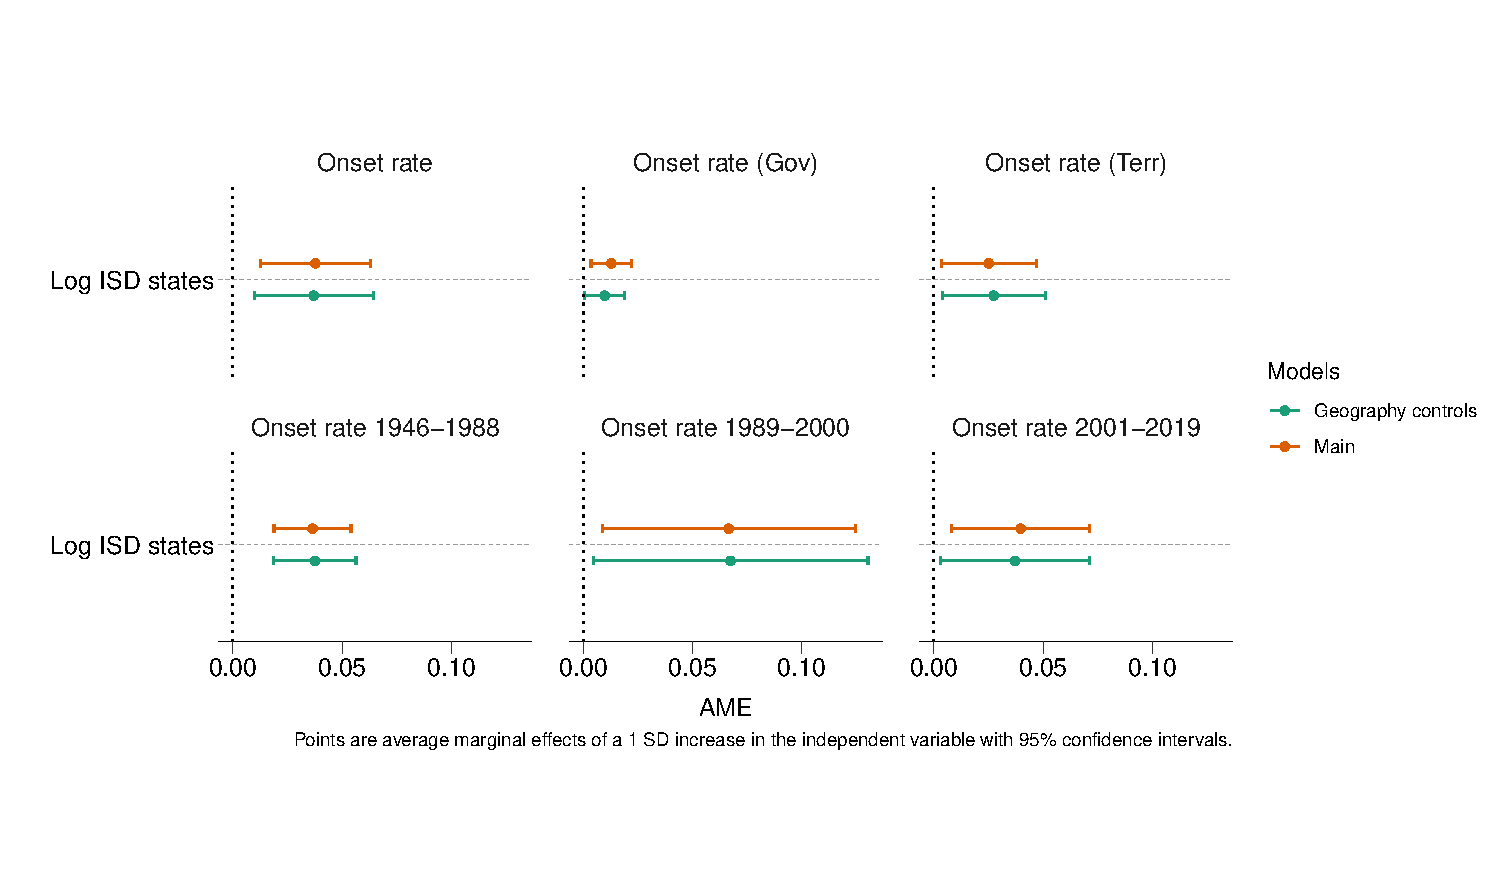
\includegraphics[width=\textwidth,keepaspectratio]{img/main_margins.pdf}
\caption{HSEs and Armed Conflict, Main Results} \label{Fig: Main_Margins}
\end{figure}


Figure \ref{Fig: Reg_Margins} shows the main models across regional and other
relevant sub-samples. HSEs are associated with more conflict onsets across
important subsamples where our theory should apply: former colonies, outside the
West (i.e states not in Western Europe or North America, also including
Australia and New Zealand), when we drop countries that get a `0', and in
Sub-Saharan Africa. The coefficients are positive but not significant at the
0.05 level in Latin America, MENA and Asia (the latter result may reflect the
lower number of states identified in Myanmar and India). More HSEs have a
generally negative impact across Eastern Europe and Central Asia. Wealth and
state capacity may have enabled these countries to offset any conflict inducing
impacts of HSEs, which we explore in the conditional effects. 

\begin{figure}[!htb]
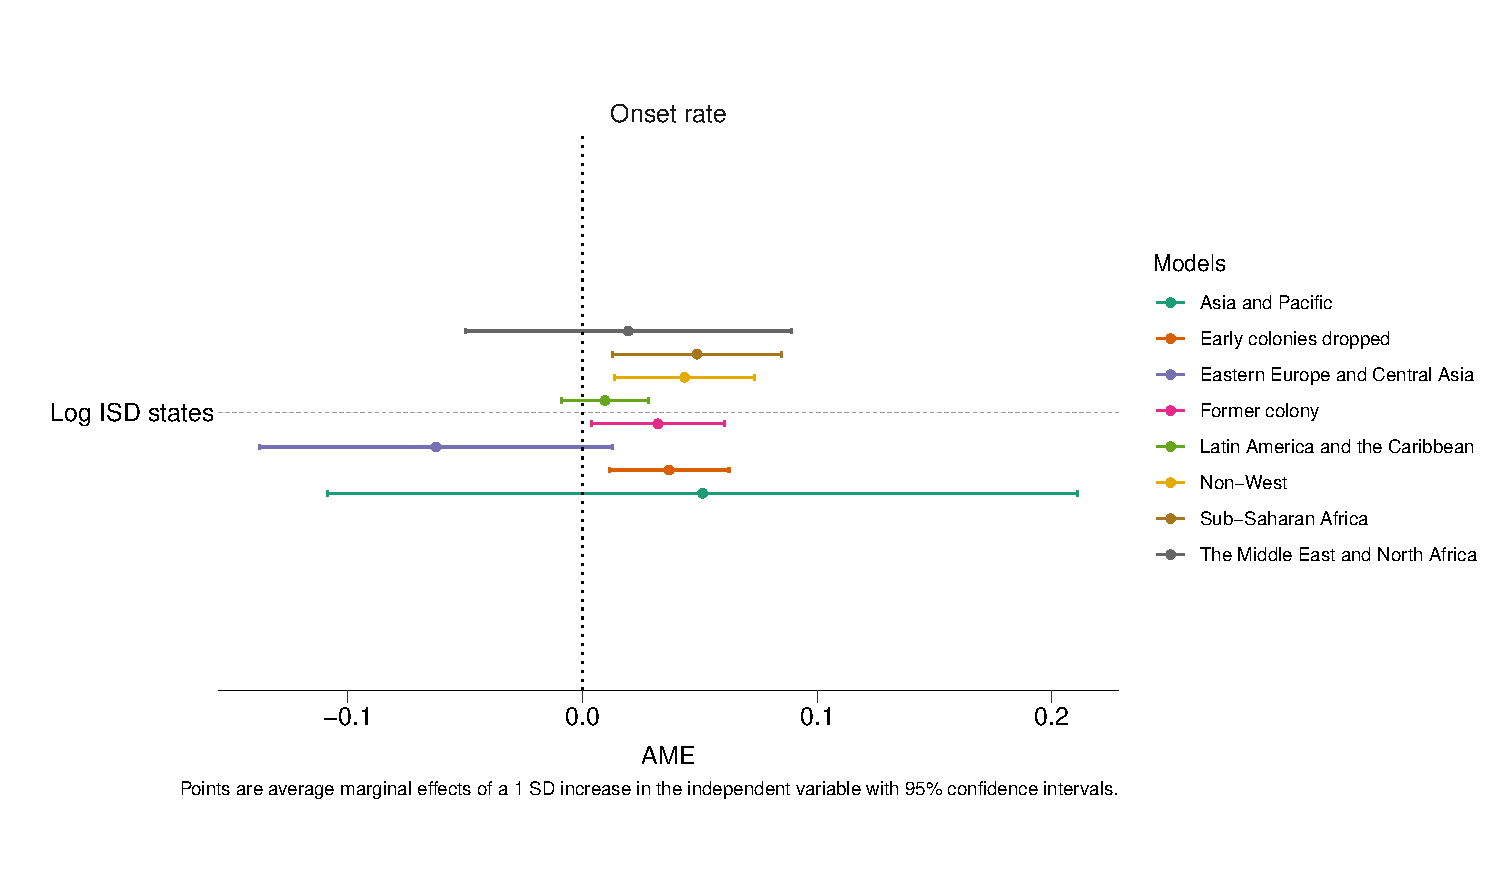
\includegraphics[width=\textwidth,keepaspectratio]{img/main_regional.pdf}
\caption{HSEs and Armed Conflict, Regional Sub-samples} \label{Fig: Reg_Margins}
\end{figure}

The results for the sub-Saharan African sub-sample are striking (regression
tables in the Appendix). We do not find a statistically significant relationship
between the average number of politically relevant ethnic groups and the number
of armed conflict onsets, while we do for the number of HSEs. This suggests that
HSEs have important, unexplored, connections to armed conflict even in regions
where ethnic politics and tensions are thought to play an influential role
\citep{Cederman2010}. This is also not simply a function of using the average
number of politically relevant EPR groups. The results are almost identical if
we use the average number of excluded EPR groups. 


\subsection{Alternative arguments}

Our mechanisms link the \emph{number} of HSEs in the territory of a modern state
to more armed conflict onsets. Similar arguments have been made in existing
studies, but that emphasise conceptually different aspects of historical or
pre-colonial statehood. In this section we adapt these arguments and test them
as alternative explanations for the HSE-conflict link. First, \citet{Paine2019}
argues that stateless ethnic groups in a state with an ethnic group that had a
pre-colonial state (SLPCS groups) rebel more frequently because of bargaining
problems and exclusionary practices by the dominant pre-colonial state ethnic
group (PCS group). Adapting this argument to a cross-sectional framework,
\citet{Paine2019}'s work suggests that the more SLPCS groups that exist in a
modern state, the more armed conflict onsets we should observe (states with no
ethnic groups that had a pre-colonial state (i.e PCS groups) also have no SLPCS
groups). As he notes, the PCS - SLPCS dynamic raises the likelihood of conflict
for all groups in a state. To measure SLPCS groups we used a count of the number
of ethnic groups in Paine's study that were at one point a SLPCS group. This
gives an estimate of the total number of `high risk' ethnic groups in the state
over the 1946-2013 period (the period of his study). We also include the number
of PCS groups. These tests are restricted to sub-Saharan Africa. 

Second, \citet{Wig2016} argues that ethnic groups with centralized pre-colonial
states can make credible commitments with the state and avoid armed conflict.
This argument is not easily adaptable to a cross-sectional framework as
\citet{Wig2016}'s study is dyadic while \textit{many} centralized pre-colonial
states might introduce additional bargaining problems that drive up the risk of
conflict for all groups, even if dyadic bargaining is easier
\citep{Cunningham2006, Walter2009}. We use the number of ethnic groups that
were centralized (a jurisdictional hierarchy score over 2) as a proportion of
all ethnic groups to re-test this argument. An ethnic demography dominated by
centralized groups (i.e Ghana) should be more conducive to peace than one
dominated by decentralized groups. 

Third, \citet{Alesina2011} emphasise that artificial borders grouped together
hostile pre-colonial groups and split others apart, which has led to low growth
and armed conflict. To test whether our results reflect
\citet{Alesina2011}'s fractal index -- which measures how `squiggly' borders are
-- we run a model including the variable from their study. 

Finally, \citet{Putterman2008, Hariri2012}, and \citet{Bockstette2012} point to
`early statehood' or state antiquity as an explanation for growth and internal
peace. Countries with a longer history of continuous statehood developed more
capable state structures that were able to generate economic growth and deter
armed conflict. While there are overlaps between state antiquity and our measure
of HSEs, our mechanisms highlight the distribution of states around or before
colonization (similar to \citet{Paine2019}), while the state antiquity data
reach further back in time. We run a model including the mean state antiquity
score from 1 A.D to 1800 in order to test whether the results for HSEs reflect a
simpler underlying relationship between early state history and conflict. Figure
\ref{Fig: SH_Margins} shows the results of models including these alternative
explanations, retaining all of the baseline controls (regional FEs are dropped
where the sample is Africa only). 

\begin{figure}[!htb]
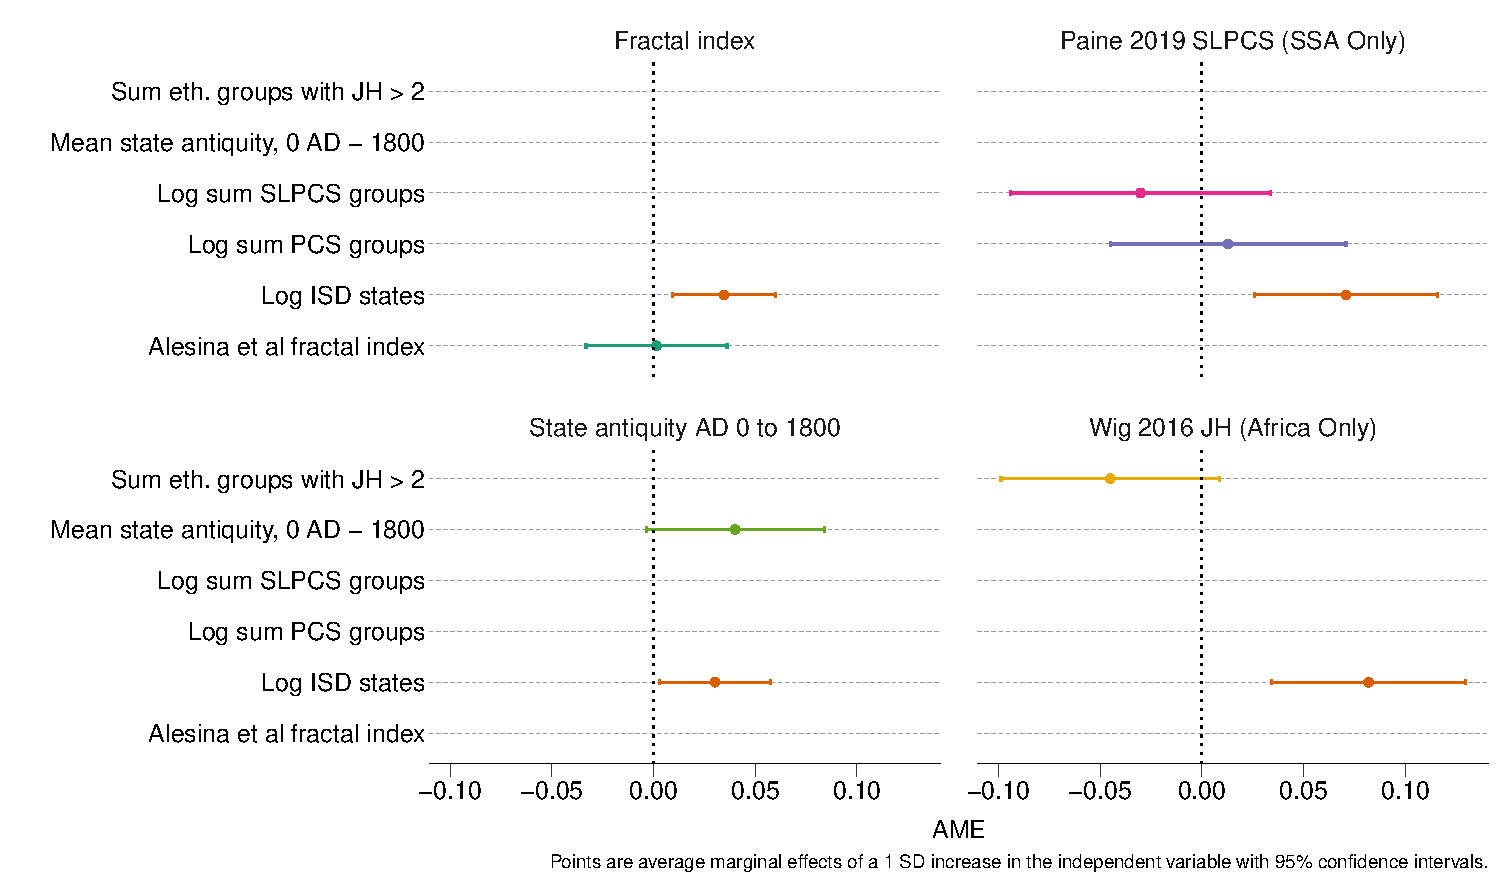
\includegraphics[width=\textwidth,keepaspectratio]{img/margins_state_history.pdf}
\caption{HSEs and Armed Conflict, Alternative explanations} \label{Fig:
SH_Margins} \end{figure}

Figure \ref{Fig: SH_Margins} shows that our main results are not simply a
reflection of the fractal index or the state-antiquity index. The coefficients
on the fractal and state-antiquity indexes have the wrong sign or are
insignificant. These models also suggest that the HSE-conflict link is not solely driven by strong, peaceful, modern states (such as Sweden) with a long history of continuous state presence that might, for other reasons, have survived into the modern world.  There is a negative but statistically insignificant relationship
between a more centralized distribution of ethnic groups and armed conflict
levels (which is not necessarily inconsistent with \citet{Wig2016}'s dyadic
argument), while HSEs remain positive and significant at the 0.05 level. More
SLPCS groups are associated with fewer armed conflict onsets, but these
coefficients are not significant at conventional levels while the HSE measure
remains significant. Overall, these models suggest that the main results are not
driven by previously identified and measured mechanisms linking pre-colonial
statehood to conflict.

%In summary, our findings suggest that there is a robust link between more HSEs
%and armed conflict onsets at the country-level in the post- WWII period. This
%association is independent of the number of politically relevant ethnic groups,
%factors conducive to state-building, historical conflict, larger states and
%region-specific effects. They are also independent of other indicators of
%past-statehood, specifically the fractal index, state antiquity, ethnic groups
%with centralized pre-colonial states and SLPCS groups. In the next section we
%turn to an initial exploration of the mechanisms that might underpin this
%relationship. 

\subsection{Mediation analysis}

Figure \ref{Fig: Mediation} shows the results of mediation models exploring
whether the HSE-conflict link can be explained by the ethnicity, weak-statehood,
or colonialism channels, or whether it is more plausibly the result of a direct
effect that we suspect is the product of mobilization networks and symbolism.
Full regression tables can be found in the appendix.

There is little evidence that variations in colonial experiences or weak
statehood transmits the relationship between HSEs and conflict. The Average
Causal Mediated Effect (ACME) for log GDP per capita in 2000 and relative tax
capacity are small and insignificant. The mean estimate is that close to 0\% of
the association can be attributed to lower GDP levels and only 2\% for relative
tax capacity. Both GDP and relative tax capacity have significant
\textit{direct} and negative associations with armed conflict. The results for
colonial exposure are similar. While more HSEs are negatively associated with
Conversionary Protestants (CPs), the mediated association is insignificant.
There is no evidence that longer periods of colonialism mediate the association
between HSEs and armed conflict.   

\begin{figure}[!htb] 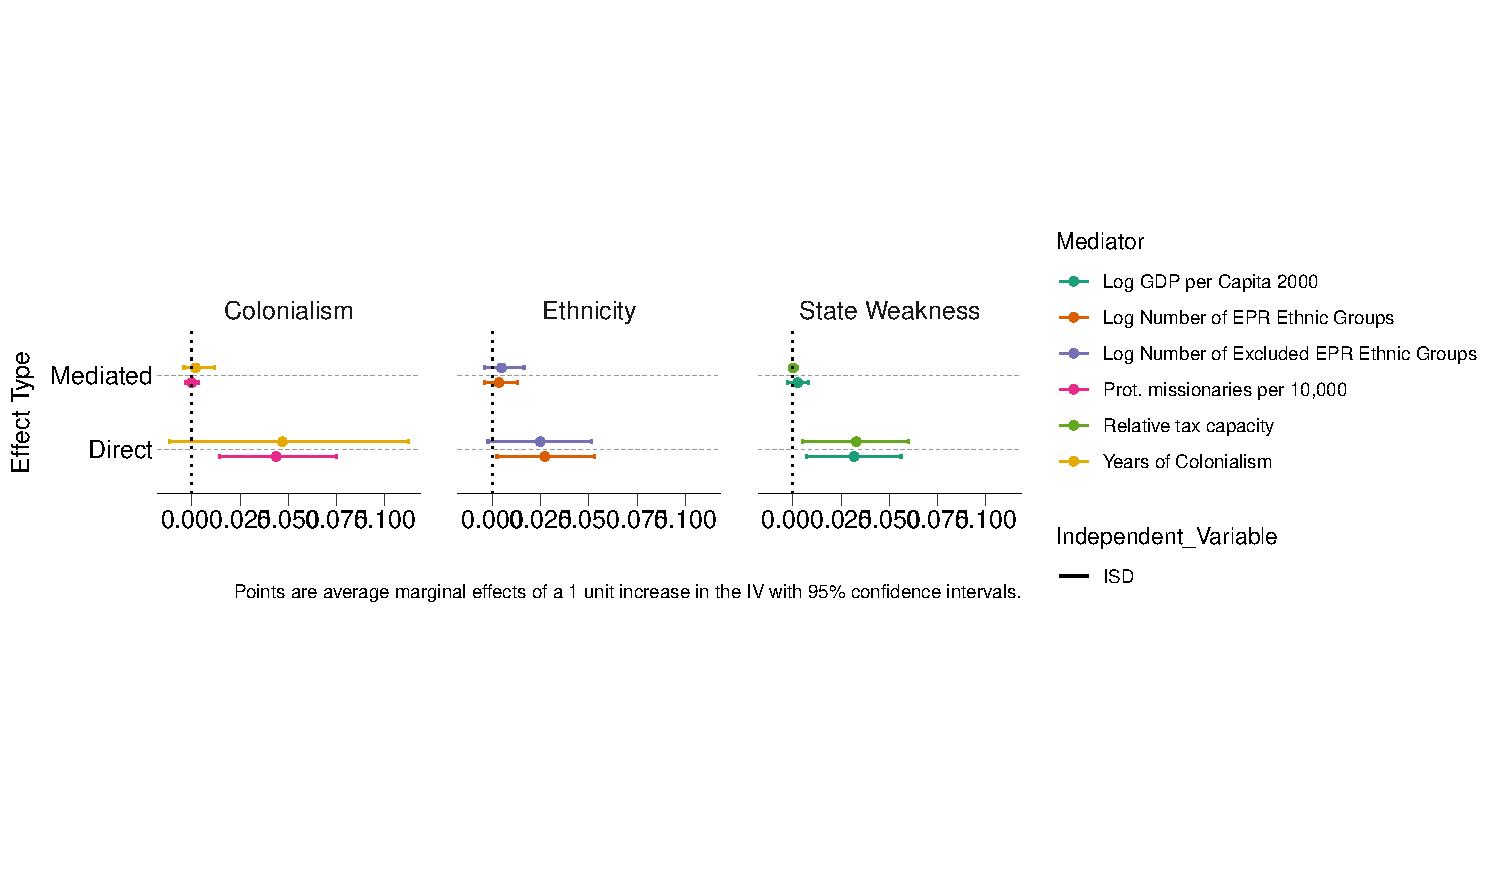
\includegraphics[width=\textwidth]{img/mediation_plot.pdf}
\caption{Mediation Analysis, Main Results} \label{Fig: Mediation} \end{figure}

There is also little evidence for the transmission of conflict through
politically relevant ethnic groups, and in all specifications there is a large
direct effect that is not explained by the ethnic channel. More HSEs are
positively associated with a higher per-year average of politically relevant EPR
groups, but this is not statistically significant in any models. Regardless of
the way we operationalize the number of politically relevant ethnic groups
across the 1946-2017 period 
%-- including the sum, maximum or level at independence, logged and unlogged,
%excluded and total -- 
there are no significant associations with more HSEs. The largest estimate is
that about 10.6\% of the association between HSEs and armed conflict runs
through more EPR ethnic groups, but this mediated effect is not statistically
significant. 

We also tested for an effect mediated by the average number of excluded ethnic
groups over the 1946-2017 period and the average size of the ethnically excluded
population, but found little evidence a mediated effect. The number of EPR
groups, the number of excluded EPR groups and the average size of ethnically
excluded populations all have strong \emph{direct} effects on armed conflict
levels in line with existing literature \citep{Buhaug2014, Cederman2010,
Cederman2013}, but there is little evidence that these effects are mediated
though more HSEs. Our results suggest that HSEs and EPR groups are related to
conflict through \textit{distinct} paths, where far less is understood about the
HSE-conflict link. This direct association may be evidence of the network and
symbolism mechanisms at work. Finally, the mediation models act as additional
robustness tests. In all of the second-stage equations that estimate the impact
of our treatment (HSEs) and mediators on armed conflict onsets, the coefficient
for HSEs remains positive and significant at the 0.01 level. The HSE-conflict
link is probably not also explained away by excluded EPR ethnic groups, modern
levels of development or differential exposure to European colonialism. 

\subsection{Conditional effects}

Figure \ref{Fig: Int_GDP} and  Figure \ref{Fig: Int_Dist} show the results of
models testing whether the impact of more
HSEs is mediated by the distance of those historical states from the capital, or
the baseline level of development that was inherited by the state in the modern
period. 

\begin{figure}[!htb] 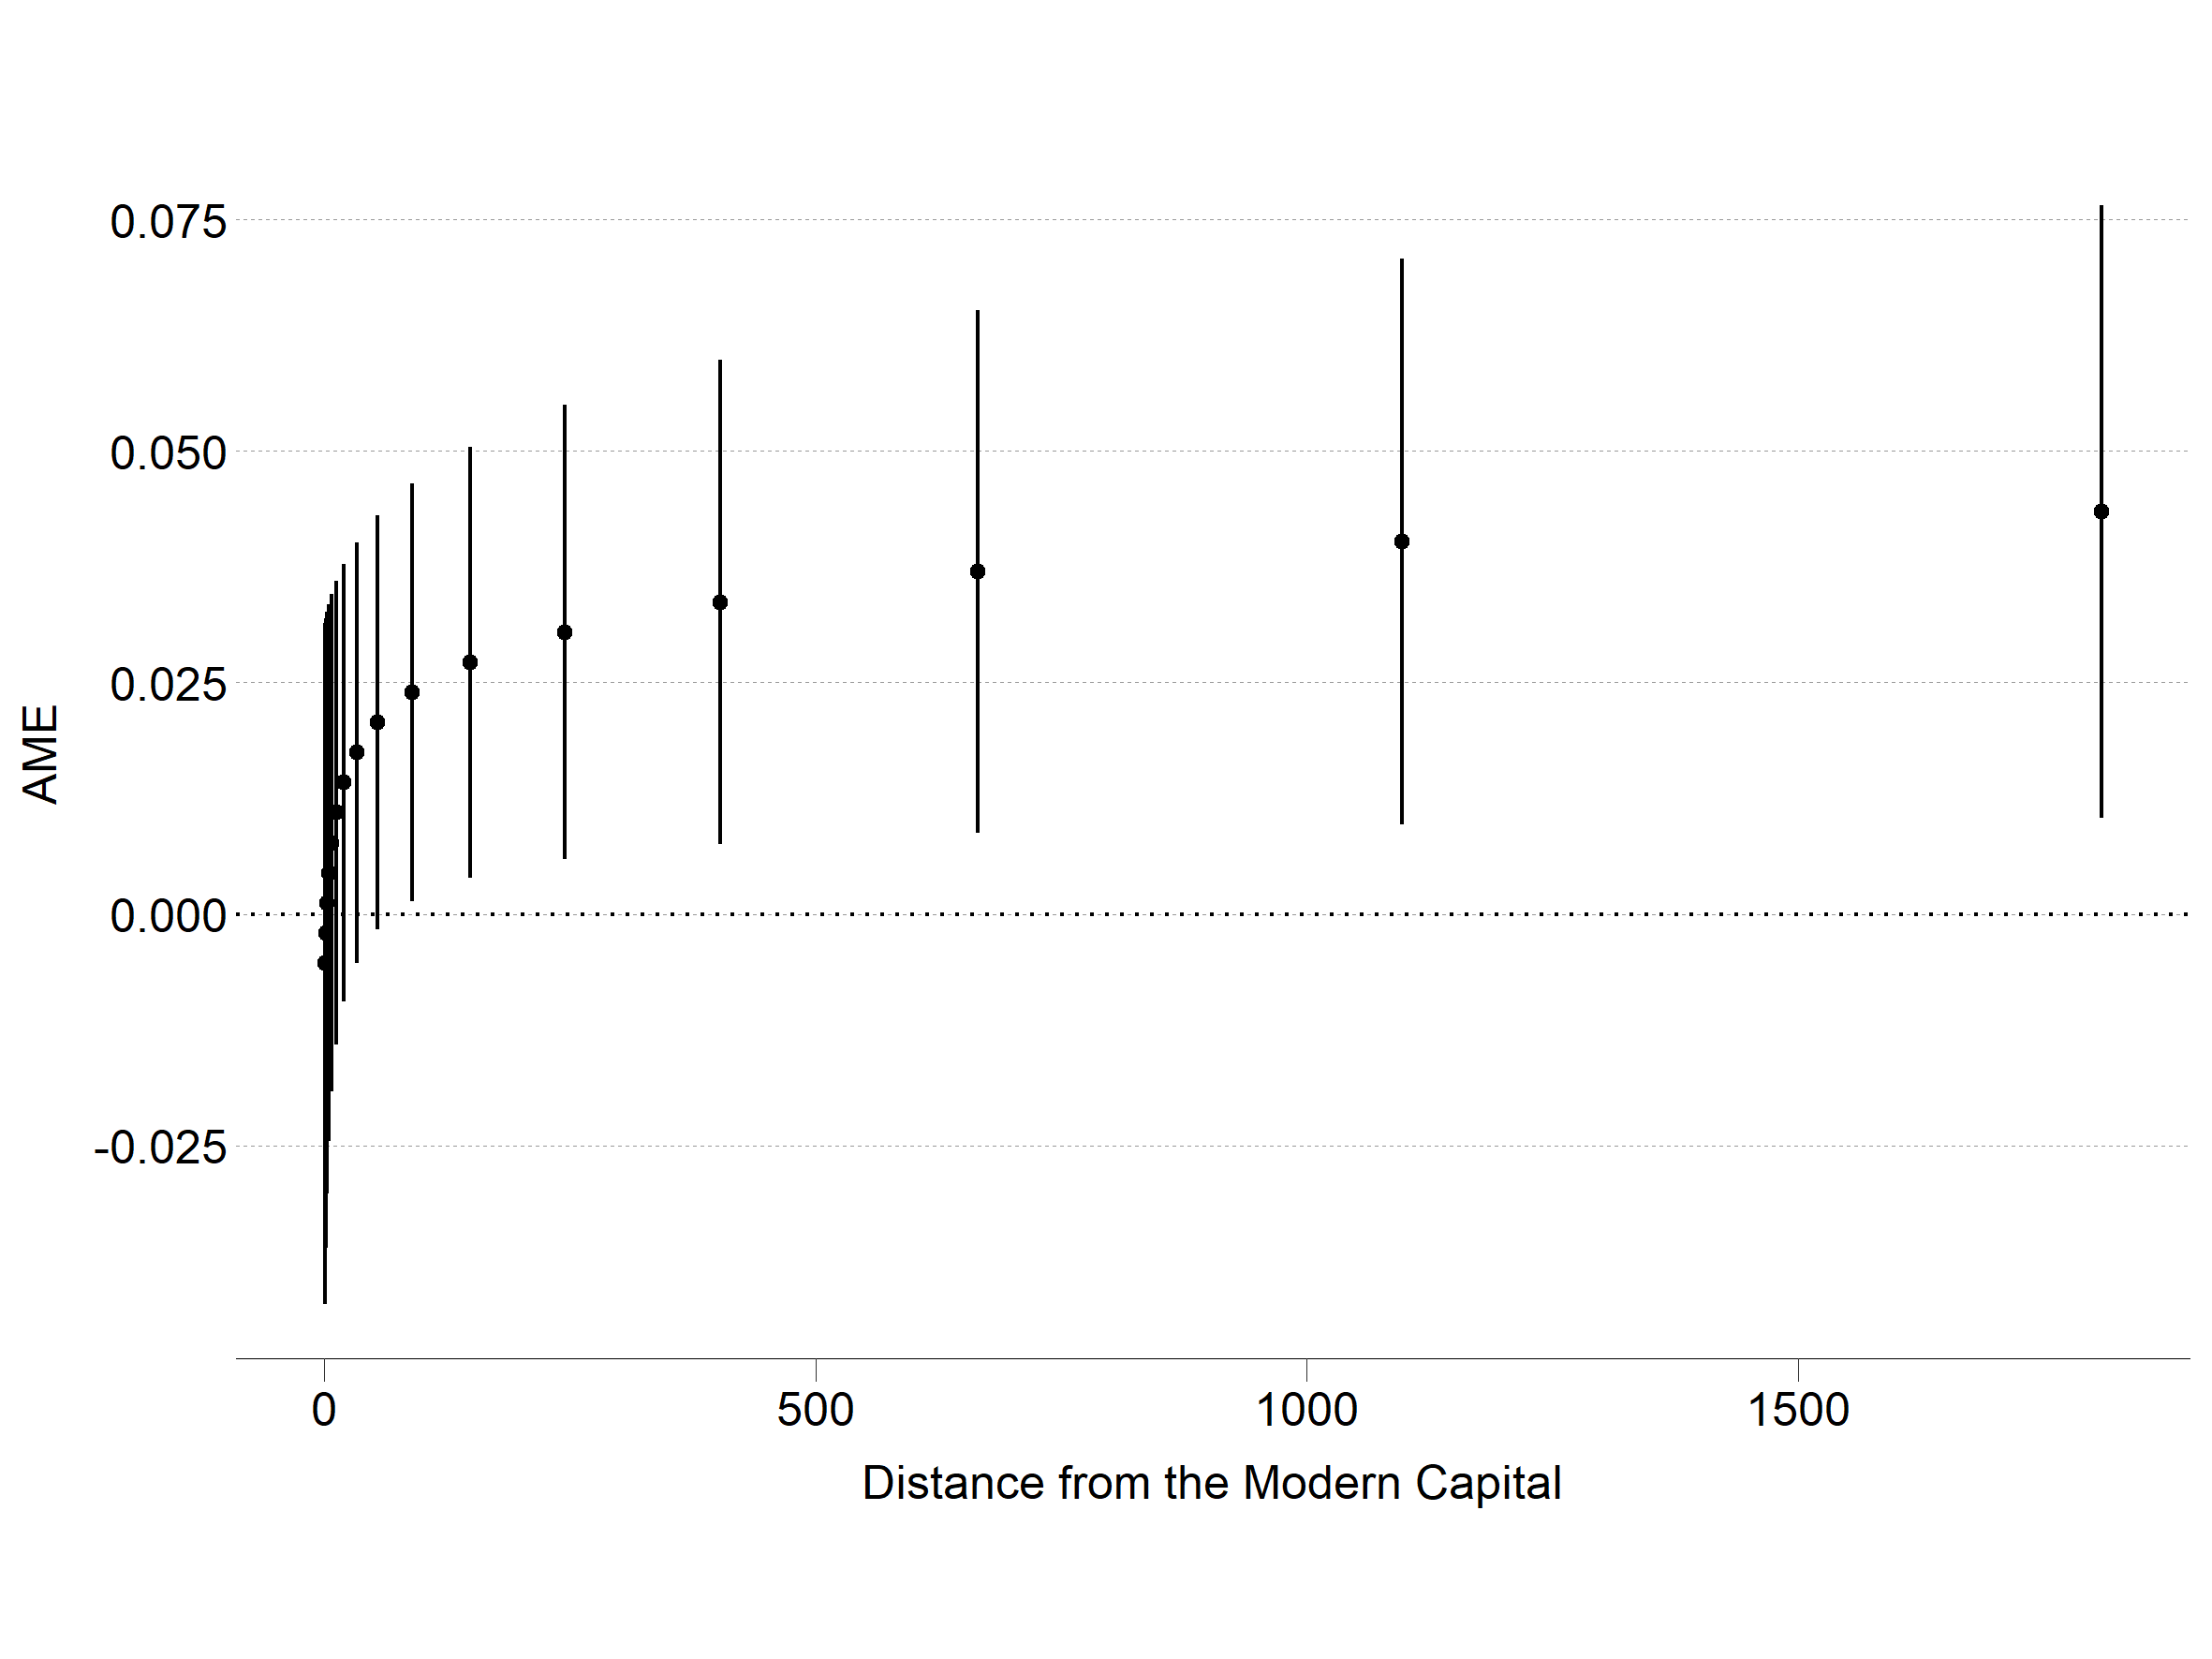
\includegraphics[width=1\textwidth]{img/dist_interaction.png}
\caption{HSEs and Conflict by mean distance from modern capital} \label{Fig:
Int_Dist} \end{figure}

\begin{figure}[!htb] 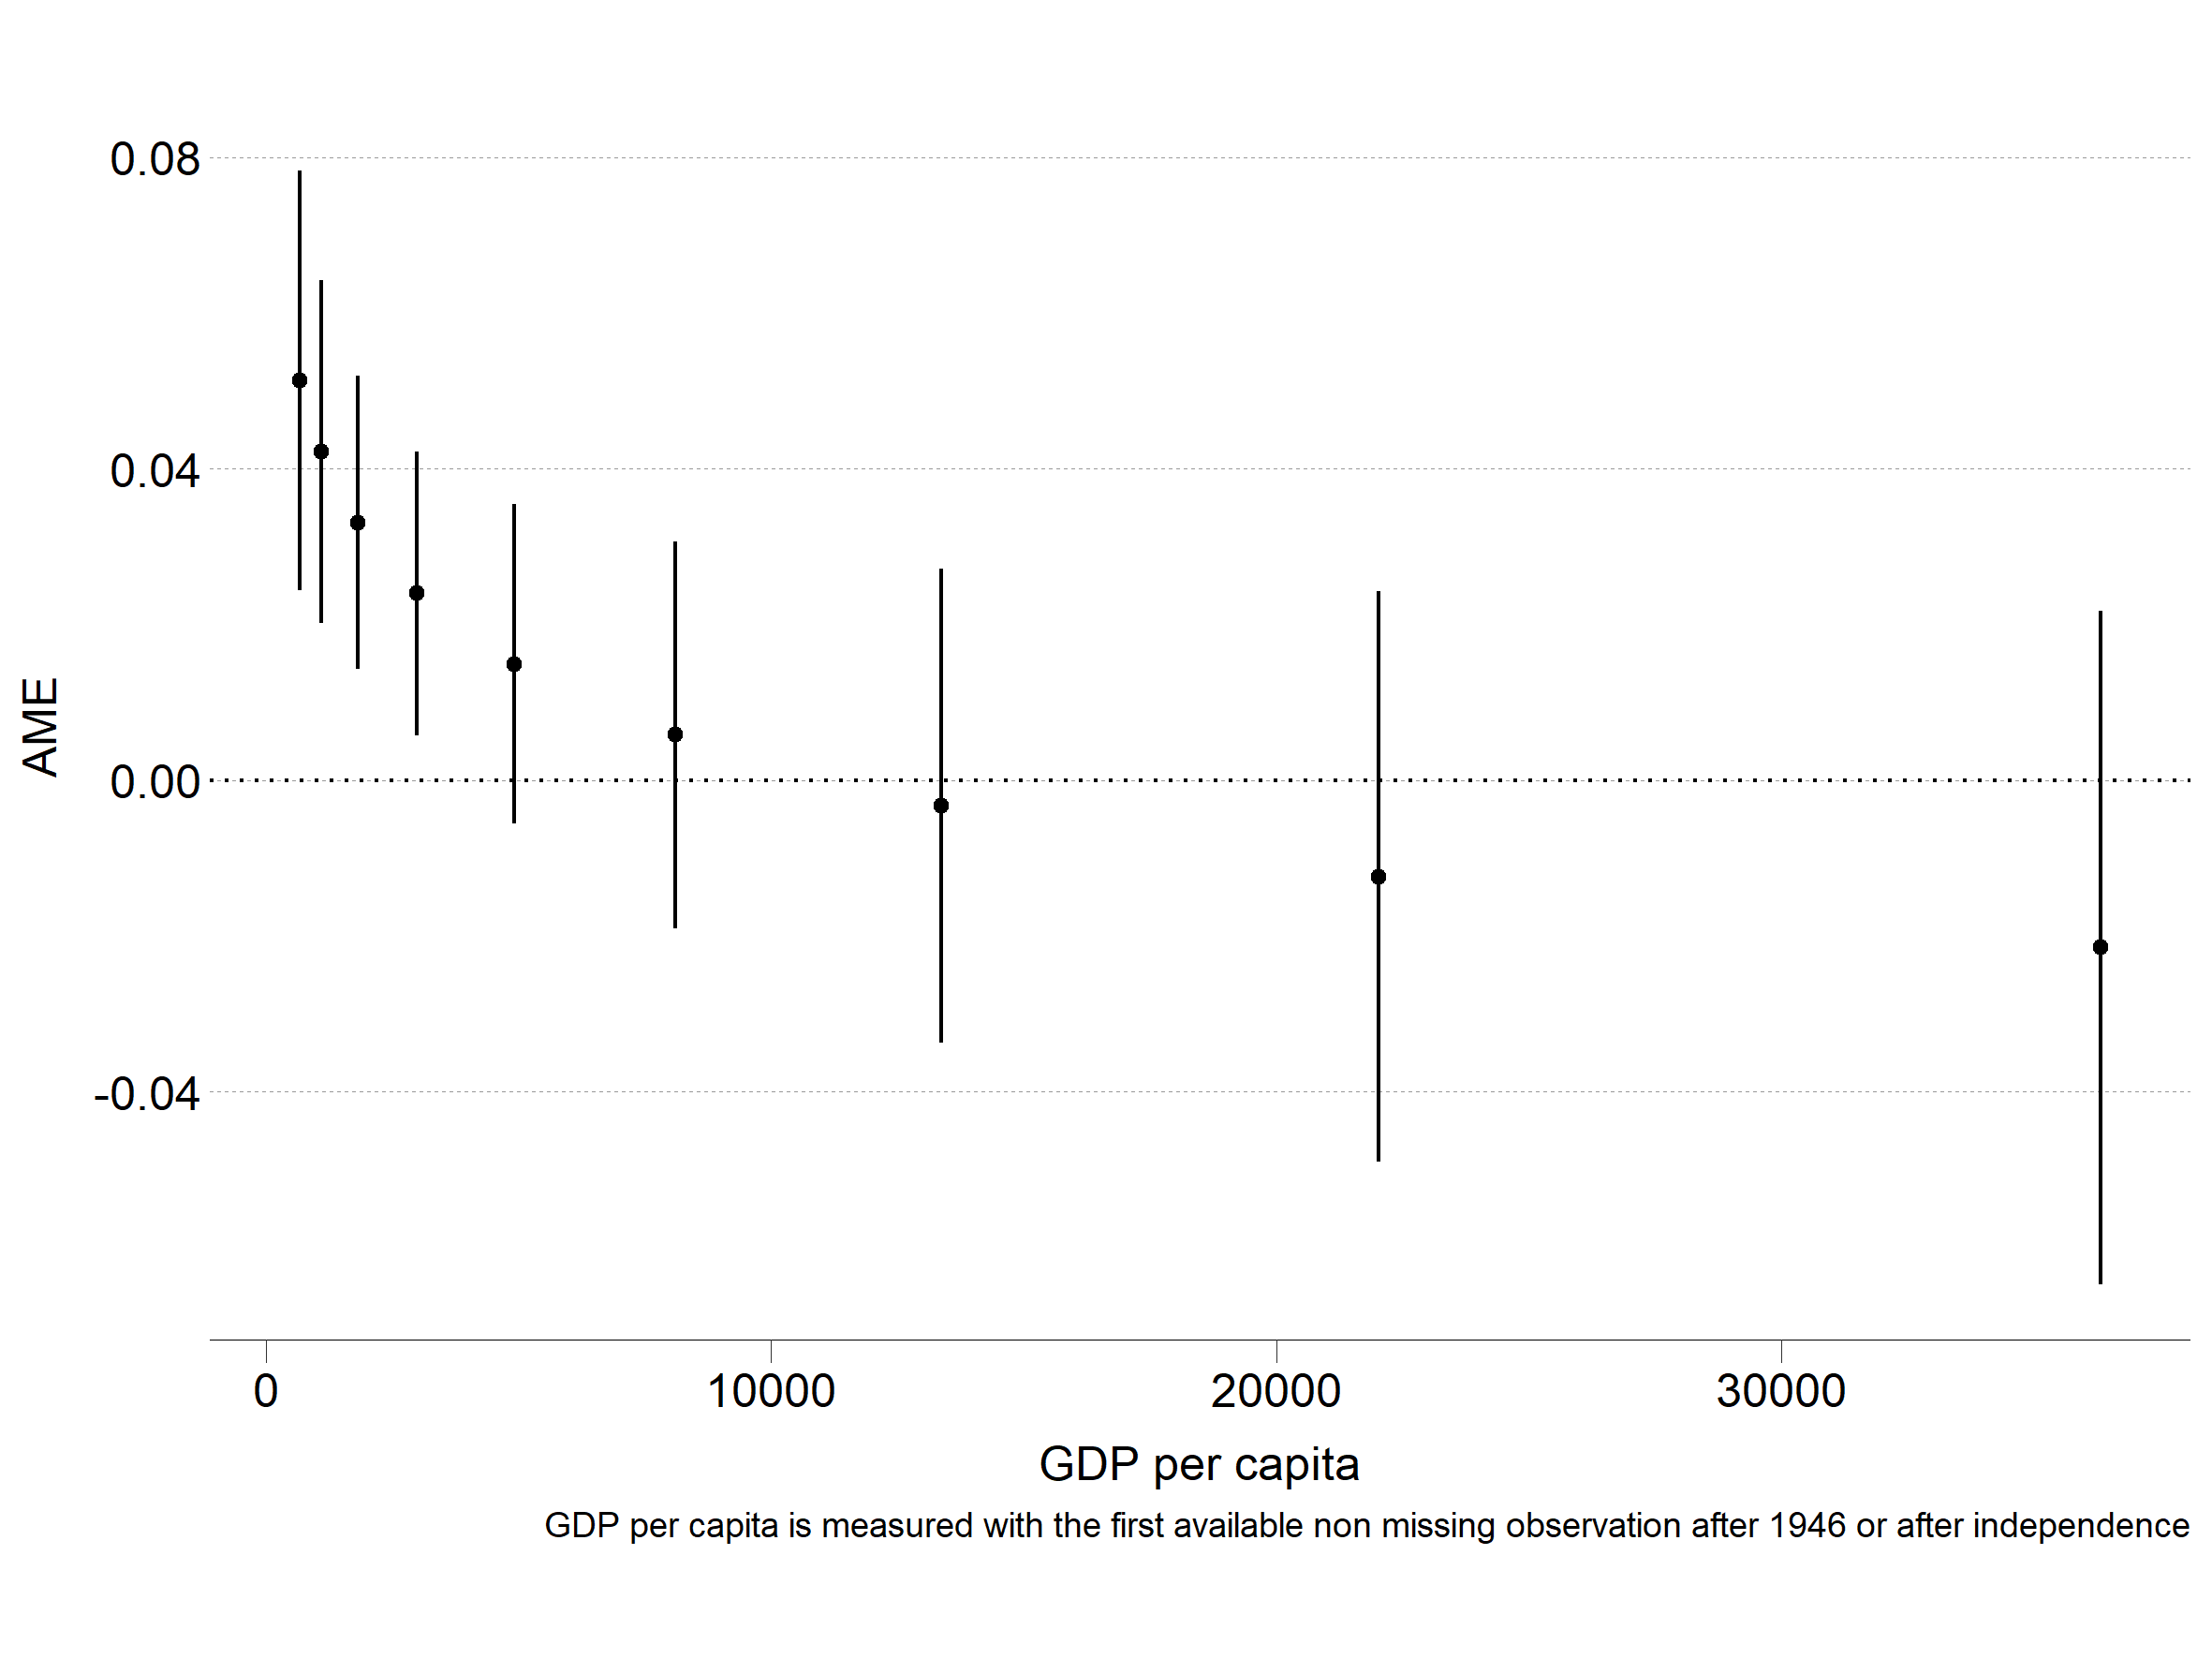
\includegraphics[width=1\textwidth]{img/gdp_interaction.png}
\caption{HSEs and Conflict by GDP per capita} \label{Fig: Int_GDP} \end{figure}


The results suggest that HSEs have stronger impacts on armed conflict onsets
when HSEs are -- on average -- located further from the modern capital. When HSEs are located close to the capital (including situations where the modern
state inherits a historical state, such as Thailand), they do not
significantly increase conflict risk. As more HSEs are located further from the capital, however, the expected
onset rate for the 1946-2019 period significantly increases. 

On the other hand, HSEs are associated with more conflict onsets when the modern
state is poorer in terms of GDP per capita. HSEs do not appear to have a
statistically significant impact on conflict onsets at higher levels of GDP per
capita, which helps explain why Italy and Germany have no recorded conflict
onsets, but were home to a large number of independent states between 1816-1939. 

Overall, these results suggest that while more HSEs may not have led to conflict
by \textit{making} states poorer (as indicated by the mediation models), HSEs
likely presented modern states with significant state building challenges where
they were located in the periphery and governance is expensive, and where states
had fewer economic resources or state capacity to effectively integrate older
states. This is also consistent with the effect of HSEs being most pronounced in
the 1946-1988 period, when many fledgling states were emerging from
colonisation with limited capacities.

\section{Conclusion}

Studies of historical statehood and conflict have focused on ethnic groups'
differing experiences of statehood. On the surface, our results may appear to
contradict existing studies that link pre-colonial statehood to domestic
\emph{peace} in   the post-colonial era \citep{Wig2016, Depetris-Chauvin2016}.
However, it may be the case that pre-colonial statehood facilitates governance
by enabling newly formed states to make credible commitments with ethnic groups
\citep{Wig2016} or by leaving behind institutional structures that can lower the
costs of governance and provide order \citep{Depetris-Chauvin2016}. However,
capacity for mobilization and governance, independent of the state, can be a
double edged sword. Our study suggests that pre-existing governance and
mobilization structures that inhere in historical states can be turned against
the state when the  \emph{number} of HSEs states that the regime has to bargain
with increases. This could be because the likelihood of bargaining failures,
miscalculation and war also increases \citep{Fearon1995, Walter2009,
Cunningham2006}. For example, in a modern state such as Ghana or Benin, where
the Ansante kingdom and the Dahomey kingdom broadly overlapped with modern
borders, the state can leverage these pre-colonial structures to facilitate
peaceful rule. Nigeria is also host to historical states, but the larger number
of states may have compounded bargaining problems to such an extent that any
advantages provided by pre-colonial statehood break down. 

A more important contribution of our study, however, is to identify links
between historical states and modern levels of armed conflict that are not
easily attributable the mechanisms that run through ethnic power relations in
the post-colonial world. We suspect that the independent effect of HSEs on civil
conflict come from the mobilization infrastructures and symbols of independent
statehood that historical states leave behind which can be used by conflict
entrepreneurs to mobilize.  Networks of rebellion need not be ethnic networks
\citep{Staniland2014} and HSEs can create networks of religious followers or
elite networks that survive the colonial experience and exist in the modern
state system. Rebel groups mobilise from a diverse array of social bases; only
half of the rebel groups in the Foundations of Rebel Groups Emergence (FORGE)
data have links to ethnic groups \citep{Braithwaite2020}, while another 20\%
have roots in religious groups and this is a growing proportion
\citep{Svensson2019}. Others emerge from political parties, student groups,
military defectors and political movements, among others. Alternatively, in
situations of material deprivation or grievance, historical states can provide
powerful touchstones of past sovereignty upon which to construct narratives that
magnify unjust oppression and create a legal basis for demands for independence
\citep{Ahram2019, Shelef2016}. We don't mean to imply that ethnicity is not
important, it clearly was important to historical state-building
\citep{Herbst2014} and modern conflict \citep{Cederman2013}, but our paper
suggests that the historical states can impact conflict levels independent of
their ability to make, or be made by, ethnic groups. 

Of course, the direct association we observe here may still reflect omitted
variable bias or another mechanism that we have not identified in this study.
The conclusions that we draw are suggestive, but we argue push the research
frontier forwards by identifying a puzzling direct effect, and specifying
mechanisms that are likely to explain it, that can from the basis for a future
research agenda. 
    
\clearpage 
\bibliographystyle{apsr} 
\bibliography{../ArtificialBorders.bib}
\clearpage 

\section{Appendix}

\subsection{Main Results: Armed conflict onset rate}

    \import{img/}{Onsets}
    
\clearpage    

\subsection{Main Results: Armed conflict onset rate, Government}

    \import{img/}{Onsets_gov}
    
        
\clearpage    
  
\subsection{Main Results: Armed conflict onset rate, Territory}

    \import{img/}{Onsets_terr}
    
    
\clearpage        

\subsection{Main Results: Armed conflict onset rate, 1946-1988}

    \import{img/}{Onsets_46_88}
 
    
\clearpage     
  
\subsection{Main Results: Armed conflict onset rate, 1989-2000}

    \import{img/}{Onsets_89_00}
    
    
\clearpage    


\subsection{Main Results: Armed conflict onset rate, 2001-2019}

    \import{img/}{Onsets_01_19}
    
    
\clearpage    

\subsection{Alternative Measures of State History}

    \import{img/}{sh_models}
    
\clearpage    

\subsection{Regional Subsets}

    \import{img/}{Onsets_Regional_ISD}
    
\clearpage    

\subsection{First Stage Mediation Equations}

    \import{img/}{med_models.tex}
    
\clearpage
 
\subsection{Second Stage Mediation Equations}

\clearpage
    \import{img/}{med_2_models.tex}
\clearpage  
 

\subsection{Models with alternative dependent variables}



    \import{img/}{alt_dvs.tex}
\clearpage  


\subsection{Sensitivity test}

Figure \ref{Fig: Sens} shows how much of the variance in the conflict onset rate and the number of HSEs a potential omitted variable would have to explain in order to render the results insignificant at the $p<0.05$ level. While similar to an Imbens test, \citet{Cinelli2020} point to several important differences. This test was run on the model using the main control variables, including region fixed effects. Not even a confounder with three times the strength of the mean number of EPR ethnic groups would render the HSE results insignificant. Any omitted confounder would have to be several times stronger than the best predictors of conflict and HSEs in our models.

% This is cool, but a lot of text gets bundled on top of each other and sometimes falls outside the graph for the ln_total_epr_groups_mean. Any way you can fix that?

    \begin{figure}[!htb] \hspace{-0,5cm} 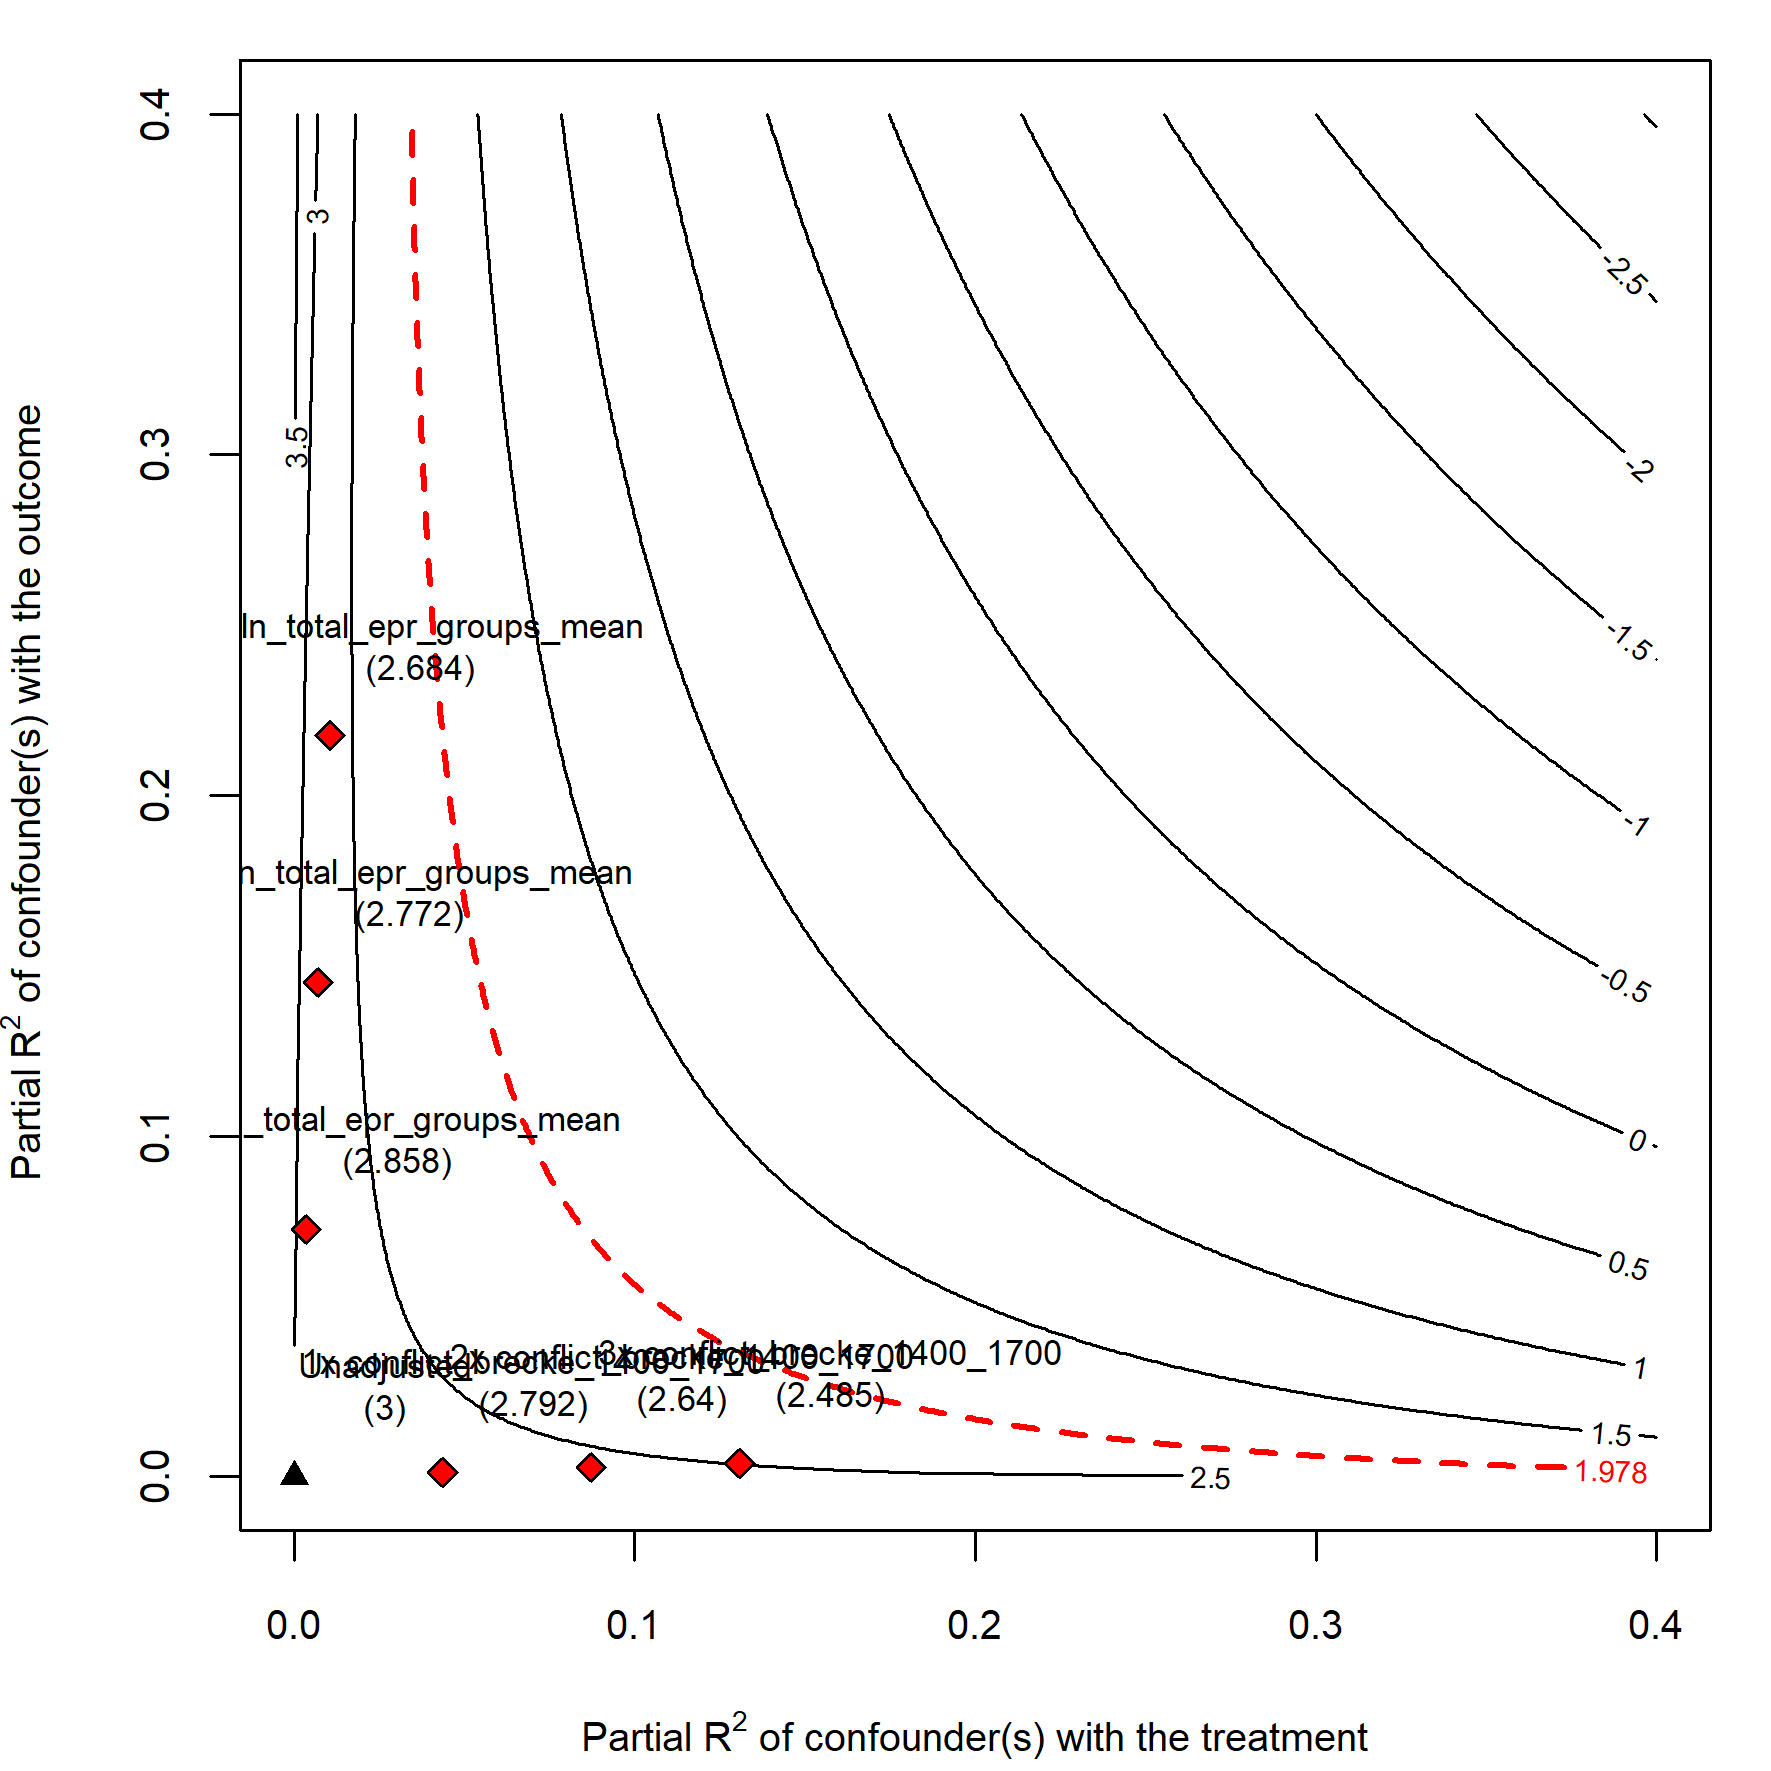
\includegraphics[width=\textwidth,
    height=\textheight, keepaspectratio]{img/hse_sens_main.png} \caption{Sensitivity test} \label{Fig: Sens} \end{figure}

\subsection{Additional tests of the state weakness mechanism}

% The reference below is not working, and I can't figure out why!
Table \ref{MediationRob} shows associations between the number of ISD states and alternative measures of state weakness to further explore these mechanisms. We use the ``State authority over territory" (Territorial capacity), ``State fiscal source of revenue" (Fiscal capacity) and ``Criteria for appointment decisions in the state administration" (Administrative capacity) variables from the VDEM dataset \citep{Coppedge2021} as indicators of various dimensions of state capacity. The territorial capacity variable captures the extent to which states control their territories. Higher scores on the fiscal capacity variable indicate movements towards direct taxation of property or income. Lower scores indicate the inability to generate taxation revenue or dependence on natural resource extraction or international aid. Higher scores on the administrative capacity variable indicate movements towards an increasingly impartial recruitment to the bureaucracy based on merit rather than personal ties or patronage. We also test the average GDP level over the 1946-2018 period and the average Polyarchy score over the same period.   

Although each of these variables represents a potential alternative mediator, we only show the first-stage equations here. None of these measures of state weakness are highly correlated with the number of ISD states between 1816-1920 and thus do not represent strong contenders for mediators. Overall, we see this as an indication that the links between ISD states and modern internal conflict rates are not well explained by the state weakness mechanism, at least on the country level. 

 \clearpage     

\import{img/}{mediation_robustness_models}
    
 \clearpage     

\subsection{Secessionism}

Here we explore the extent to which the main results reflect an increase in the risk of secessionist movements. The UCDP data differentiates between conflicts with ``governmental'' and ``territorial'' incompatibilities, but does not specifically identify secessionist movements (although these are a subset of territorial conflicts). We use data from Griffiths (2016) on secessionist movements active in independent states after 1946 to unpack the relationship between HSEs and secessionism further.  


    \import{img/}{secession_table_hses}

Table \ref{Tab: Sec_Desc} shows how the onset and incidence rate vary across levels of HSE presence. The patterns are similar to the main results and those for territorial conflicts in the main paper. The onset rate is low for 0 HSEs, rising for 1 HSE (again, largely because of Myanmar), before dropping and then rising to the highest onset (and incidence) rate for states with more than 10 HSEs. Although the number of observations is small in the category of 10+ HSEs, secessionist movements in these states tend also to be more violent. 

 
Table \ref{SecTable} re-runs the main models, but using the onset rate of violent secessionist movements from \cite{Griffiths2016} as the dependent variable. Increasing numbers of HSEs are still positively associated with the onset rate of secessionist movements, but the coefficient is smaller than in the main models (for territorial conflicts) and generally less precisely estimated. We think this supports the idea that the HSE-conflict link is not only a story of secession, but also challenges over government. 
    
        \import{img/}{secession_robustness_models}

 \clearpage   
 
\subsection{Historical Conflict}

Historical conflict is an important alternative explanation for two reasons. First, historical conflict may lower trust between groups and increase the chances of modern conflict \citep{Besley2014}. On the other hand, historical conflict may reflect successful state-building, where states with higher levels of historical conflict are more stable and peaceful today because they have already eliminated rivals and established themselves as the most capable state in that territory. This latter explanation is a form of survivorship bias, where modern states with few HSEs are the product of past competition and conflict that has selected out less capable states, leaving more capable states in their wake. To an extent this latter process is a part of our argument. States that emerged after the Second World War were not formed through a more ``organic'' process of conflict and competition, but through a combination of relatively arbitrary colonial border drawing and decolonization movements. Moreover, these states entered an international system where borders were hard to revise \citep{Herbst2014}. Unlike European states that had competed with rivals for centuries prior, new states such as Nigeria, the Democratic Republic of Congo or Indonesia were established with many potential rivals, which we argue raises the probability of conflict. 

Nonetheless, we wish to separate our study about the conflict inducing effects of HSEs from a story whereby modern conflict is simply reflective of past conflict, whether in the sense that past conflict created more peaceful states, or more conflict-prone states. The variable we use in the main models to control for historical conflict come from the data produced by \citet{Dincecco2019} who link conflicts in Brecke's (1999) conflict catalogue to modern states. \citet{Dincecco2019}'a work has several advantages. First, they record conflicts going back to 1400 meaning we can measure conflict levels before the number of HSEs (which we measure in the 1816-1939 period), although many HSEs do have deeper roots in time and post-treatment bias may still be an issue with this variable. Second, the intensity threshold for inclusion in Brecke's catalogue is lower than for other datasets (The Correlates of War, Project Mars) which we think means that these data capture more conflicts in Africa and South Asia, which tend to be under-reported in other sources. 

Figure \ref{Fig: BreckeMap} shows the distribution of the historical conflict variable. 

   \begin{figure}[hpbt] \hspace{-0,5cm} 
   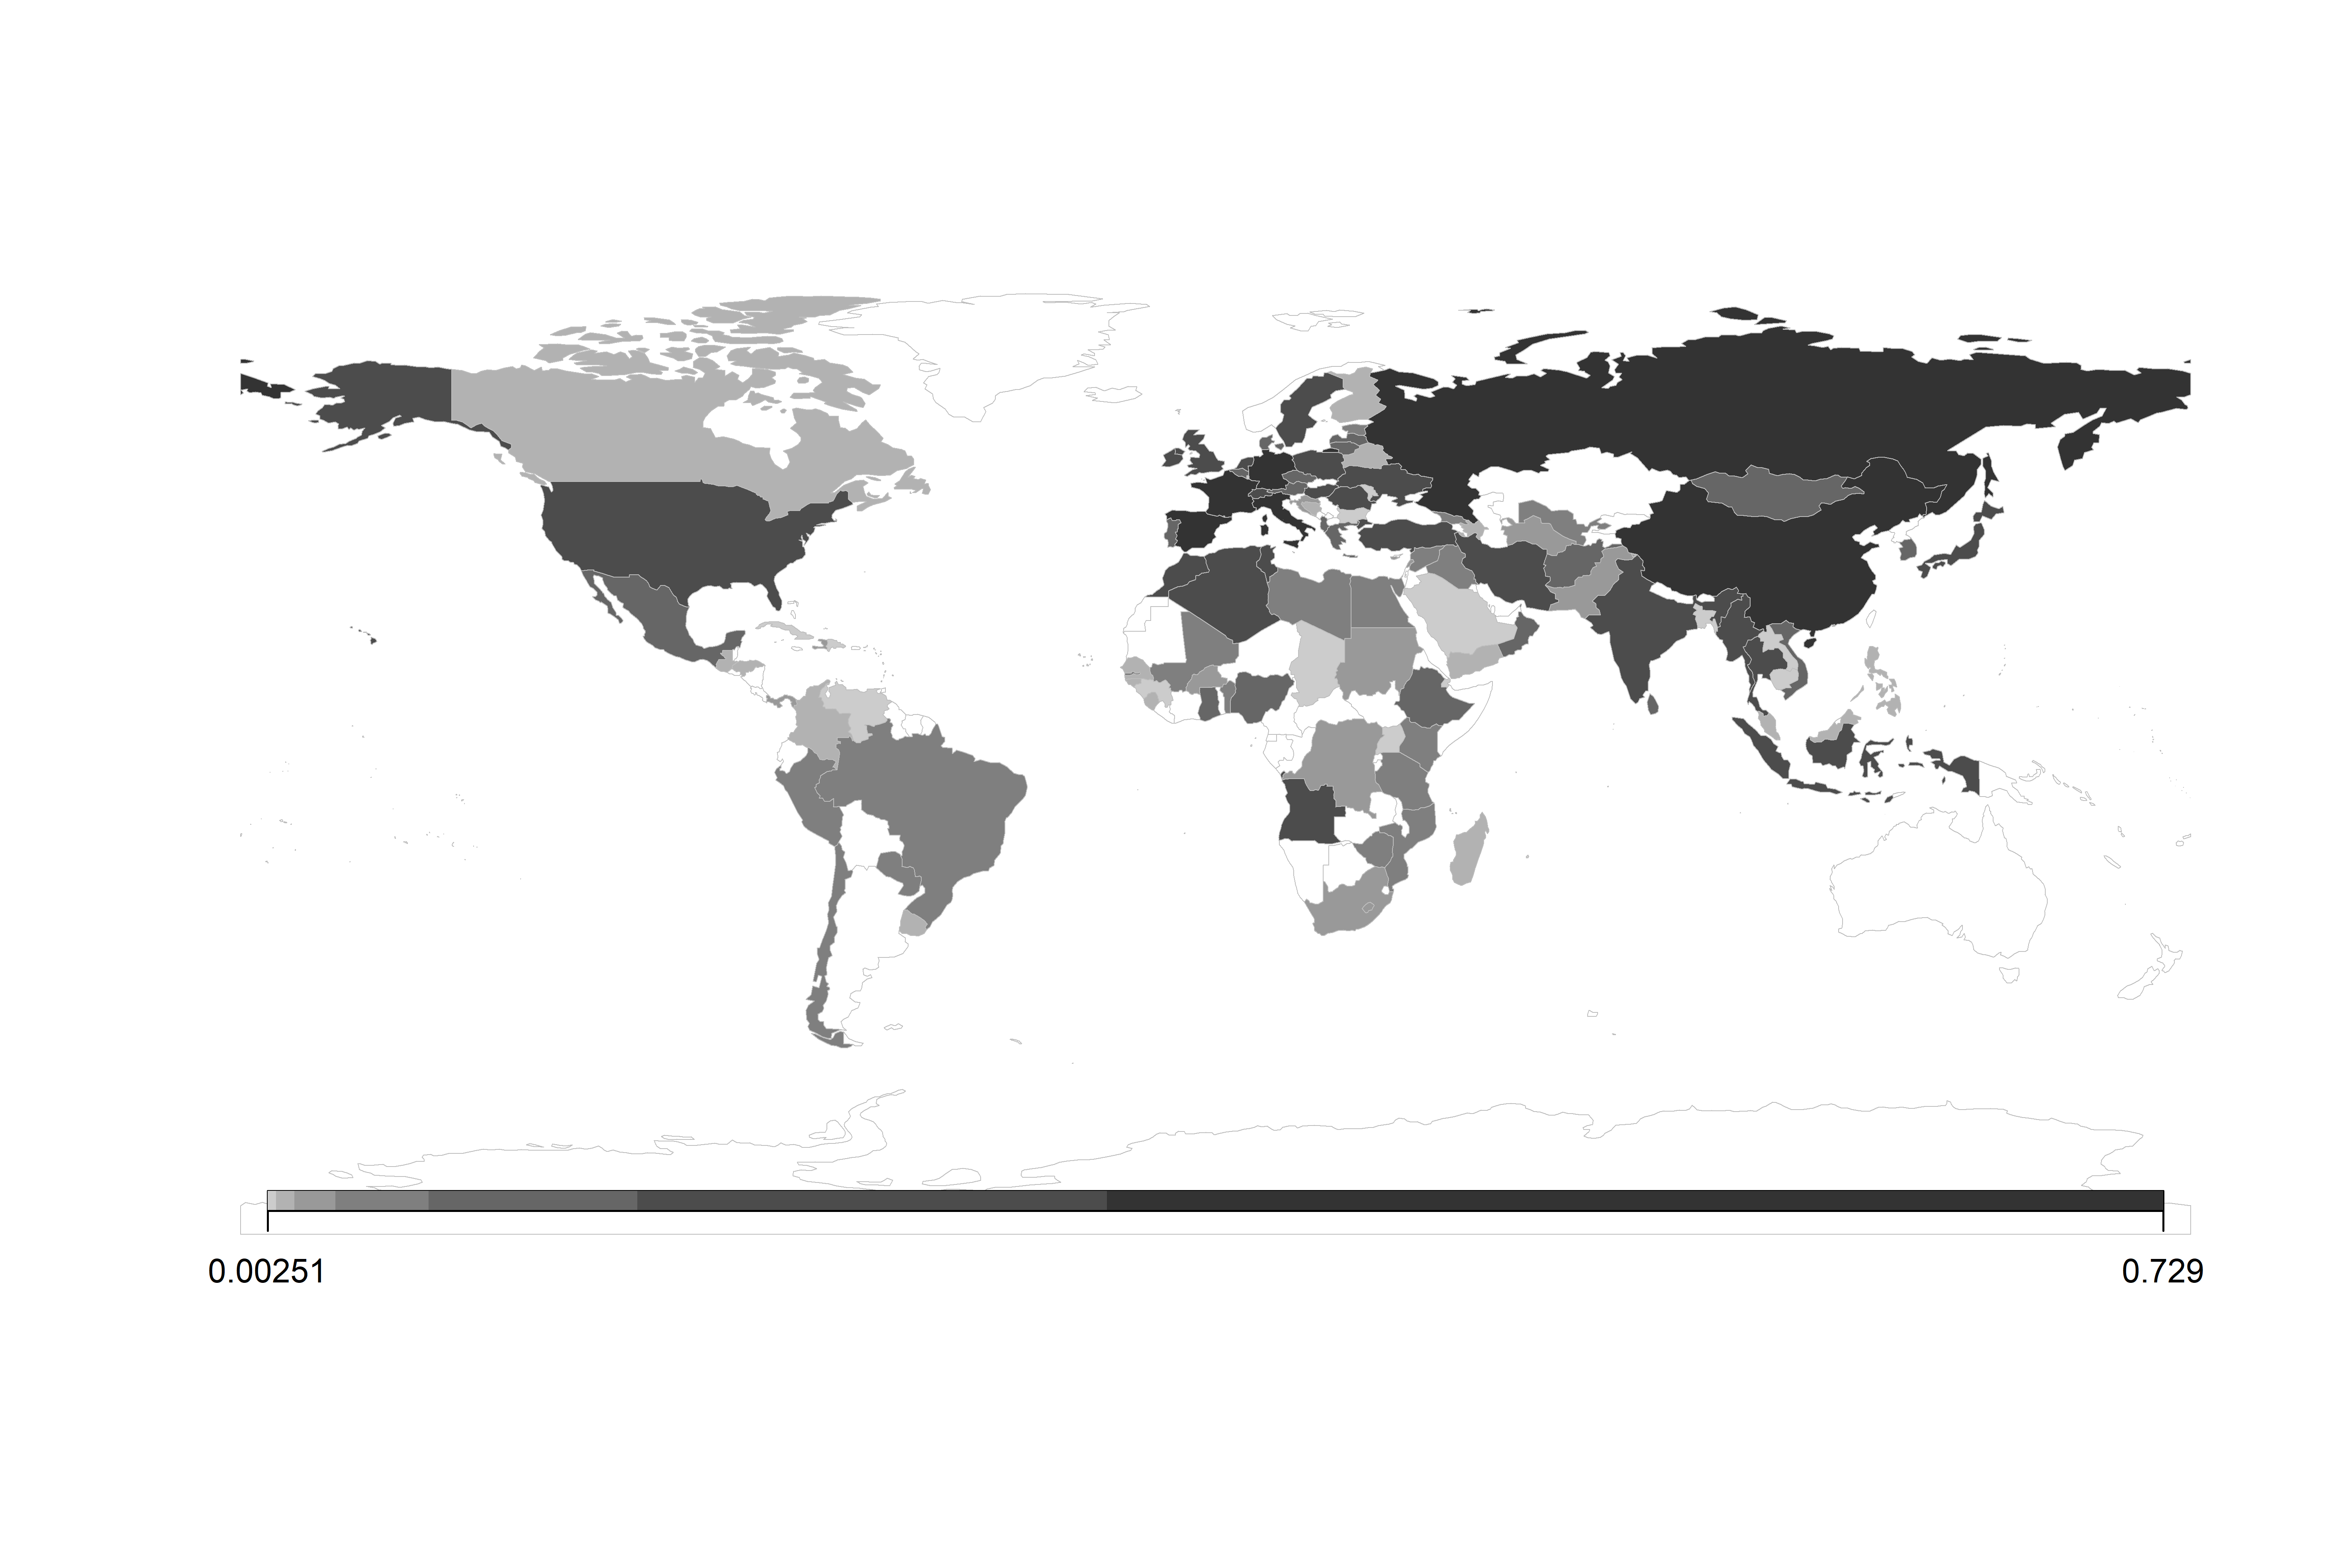
\includegraphics[width=\textwidth,
    height=\textheight, keepaspectratio]{img/historical_conflict_map.png} \caption{Historical Conflict (logged), 1400-1799} \label{Fig: BreckeMap} \end{figure}

In the main models we use the percentage of years between 1400 and 1700 as the main control, but here we test additional specifications. First, we use the raw number of conflicts in a country between 1400-1700. Second, we test the square root transformation of this variable to reduce the impact of outliers. Third, we test the square root transformed percentage of years between 1400-1700 and fourth we test the percentage of conflict years between 1400-\textbf{1799} to assess whether adding 18th century conflicts changes the results. Finally, we interact our main historical conflict control with the region fixed effects, to allow the impacts of war to vary across regions, as \citet{Dincecco2019} find in relation to state capacity. Table \ref{Tab: Hist_Conflict_Rob} shows the results of these models. Our main results are largely unchanged. Similar to \citet{Dincecco2019}, we find that historical conflict in Africa has has a significantly different association with modern conflict than in other regions. 

     \import{img/}{historical_conflict_robustness}

\clearpage

\subsubsection{Using Project Mars}

Systematically collected data on historical conflict with global coverage are rare, and Brecke's conflict catalogue and \citet{Dincecco2019}'s adaptation are the only source that we are aware of with coverage before 1800. Coverage in the 19th century is better where there are several sources that record wars during this period. Here we draw upon Project Mars (v1.1, \citep{Lyall2020}) to construct an alternative measure of historical conflict. The Project Mars data provide information on 826 different participants in conventional wars from 1800-2011. First, we subsetted the data, including only participants in wars from 1800-1900 and only participants within 1000km of the staring battle. Put differently, we are only including wars in the 19th century and only ``local'' participants in those wars.\footnote{The results are very similar if we use smaller distance thresholds, specifically, 500km and 100km} This excludes cases that would attribute a historical conflict to the United Kingdom when it was fighting in sub-Saharan Africa, for example. We then matched these participating states in Project Mars with states in the ISD data using the Statename variable. Then, we have coded the modern ``destination states'' for each participant using the information in ISD on the modern locations of ISD states. For states in \citet{Lyall2020} without a matching ISD state, we have coded the modern state in which the participant was located. For each modern state, we then calculated the total number of historical wars that involved a state on that territory. For example, if all participants in a historical war (as indicated by \textit{warnum} in \citet{Lyall2020}) were within the territory of a single modern state, that territory is attributed with one historical war. For example, the Tukolor-Bambara war of 1855 (\textit{warnum} 75) involves the Tukolor empire and the kingdom of Kaarta, both primarily based in modern day-Mali. This conflict started 425km from the capital of Tukolor and 1km from Kaarta and therefore both are retained as ``local'' participants. Since both participants are located in modern Mali, Mali is attributed with the historical conflict. Some conflicts involve ``local'' participants located in different modern states. For example the Durrani Empire and the Sikh Kingdom fought several wars between 1813 and 1822. The Durrani Empire is in modern day Afghanistan and the Sikh empire in modern-day Pakistan. Both of these states were ``local'' participants, located less than 1000km from the starting battle, and in this case, both Afghanistan and Pakistan are attributed with a historical conflict.       

This approach to measuring historical conflict has some advantages. Primarily, wars in Project Mars are linked to specific states in the ISD, meaning that if our results are best explained by historical states fighting wars then there is a closer conceptual link between states and wars using these data. Brecke, for example, includes wars that may not involve states and are less relevant to explaining the HSE-conflict link we outline in the paper. 

The main downside is that this measure introduces post-treatment bias because the wars are measured contemporaneously to statehood (i.e between 1800-1900). More wars probably occur in territories with more states to fight them and to the extent that states cause wars we are controlling for part of the association between HSEs and modern conflict. Empirically this appears to be the case as both the historical conflict indicator from \citet{Dincecco2019} and the measure based on \citet{Lyall2020} are highly correlated with the number of HSEs. Table \ref{Tab: Hist_Conf_Models} shows some simple associations between the levels of historical conflict and the number of HSEs, controlling for population density in 1500, the timing of the neolithic revolution, land area, latitude and slave exports by land area. 

     \import{img/}{hses_hist_conf}

Symbols and institutions, for example, could be more potent or established when historical states have a history of fighting conventional wars. Nonetheless, the historical conflict- modern conflict link is an alternative mechanism to our proposed mechanism and this approach represents an alternative method to account for the impacts of historical conflict that complements the analyses with the Brecke data. 

Figure \ref{Fig: Mars_Map} shows the spatial distribution of wars in the 19th century, using the data from \citet{Lyall2020}. 

   \begin{figure}[hpbt] \hspace{-0,5cm} 
   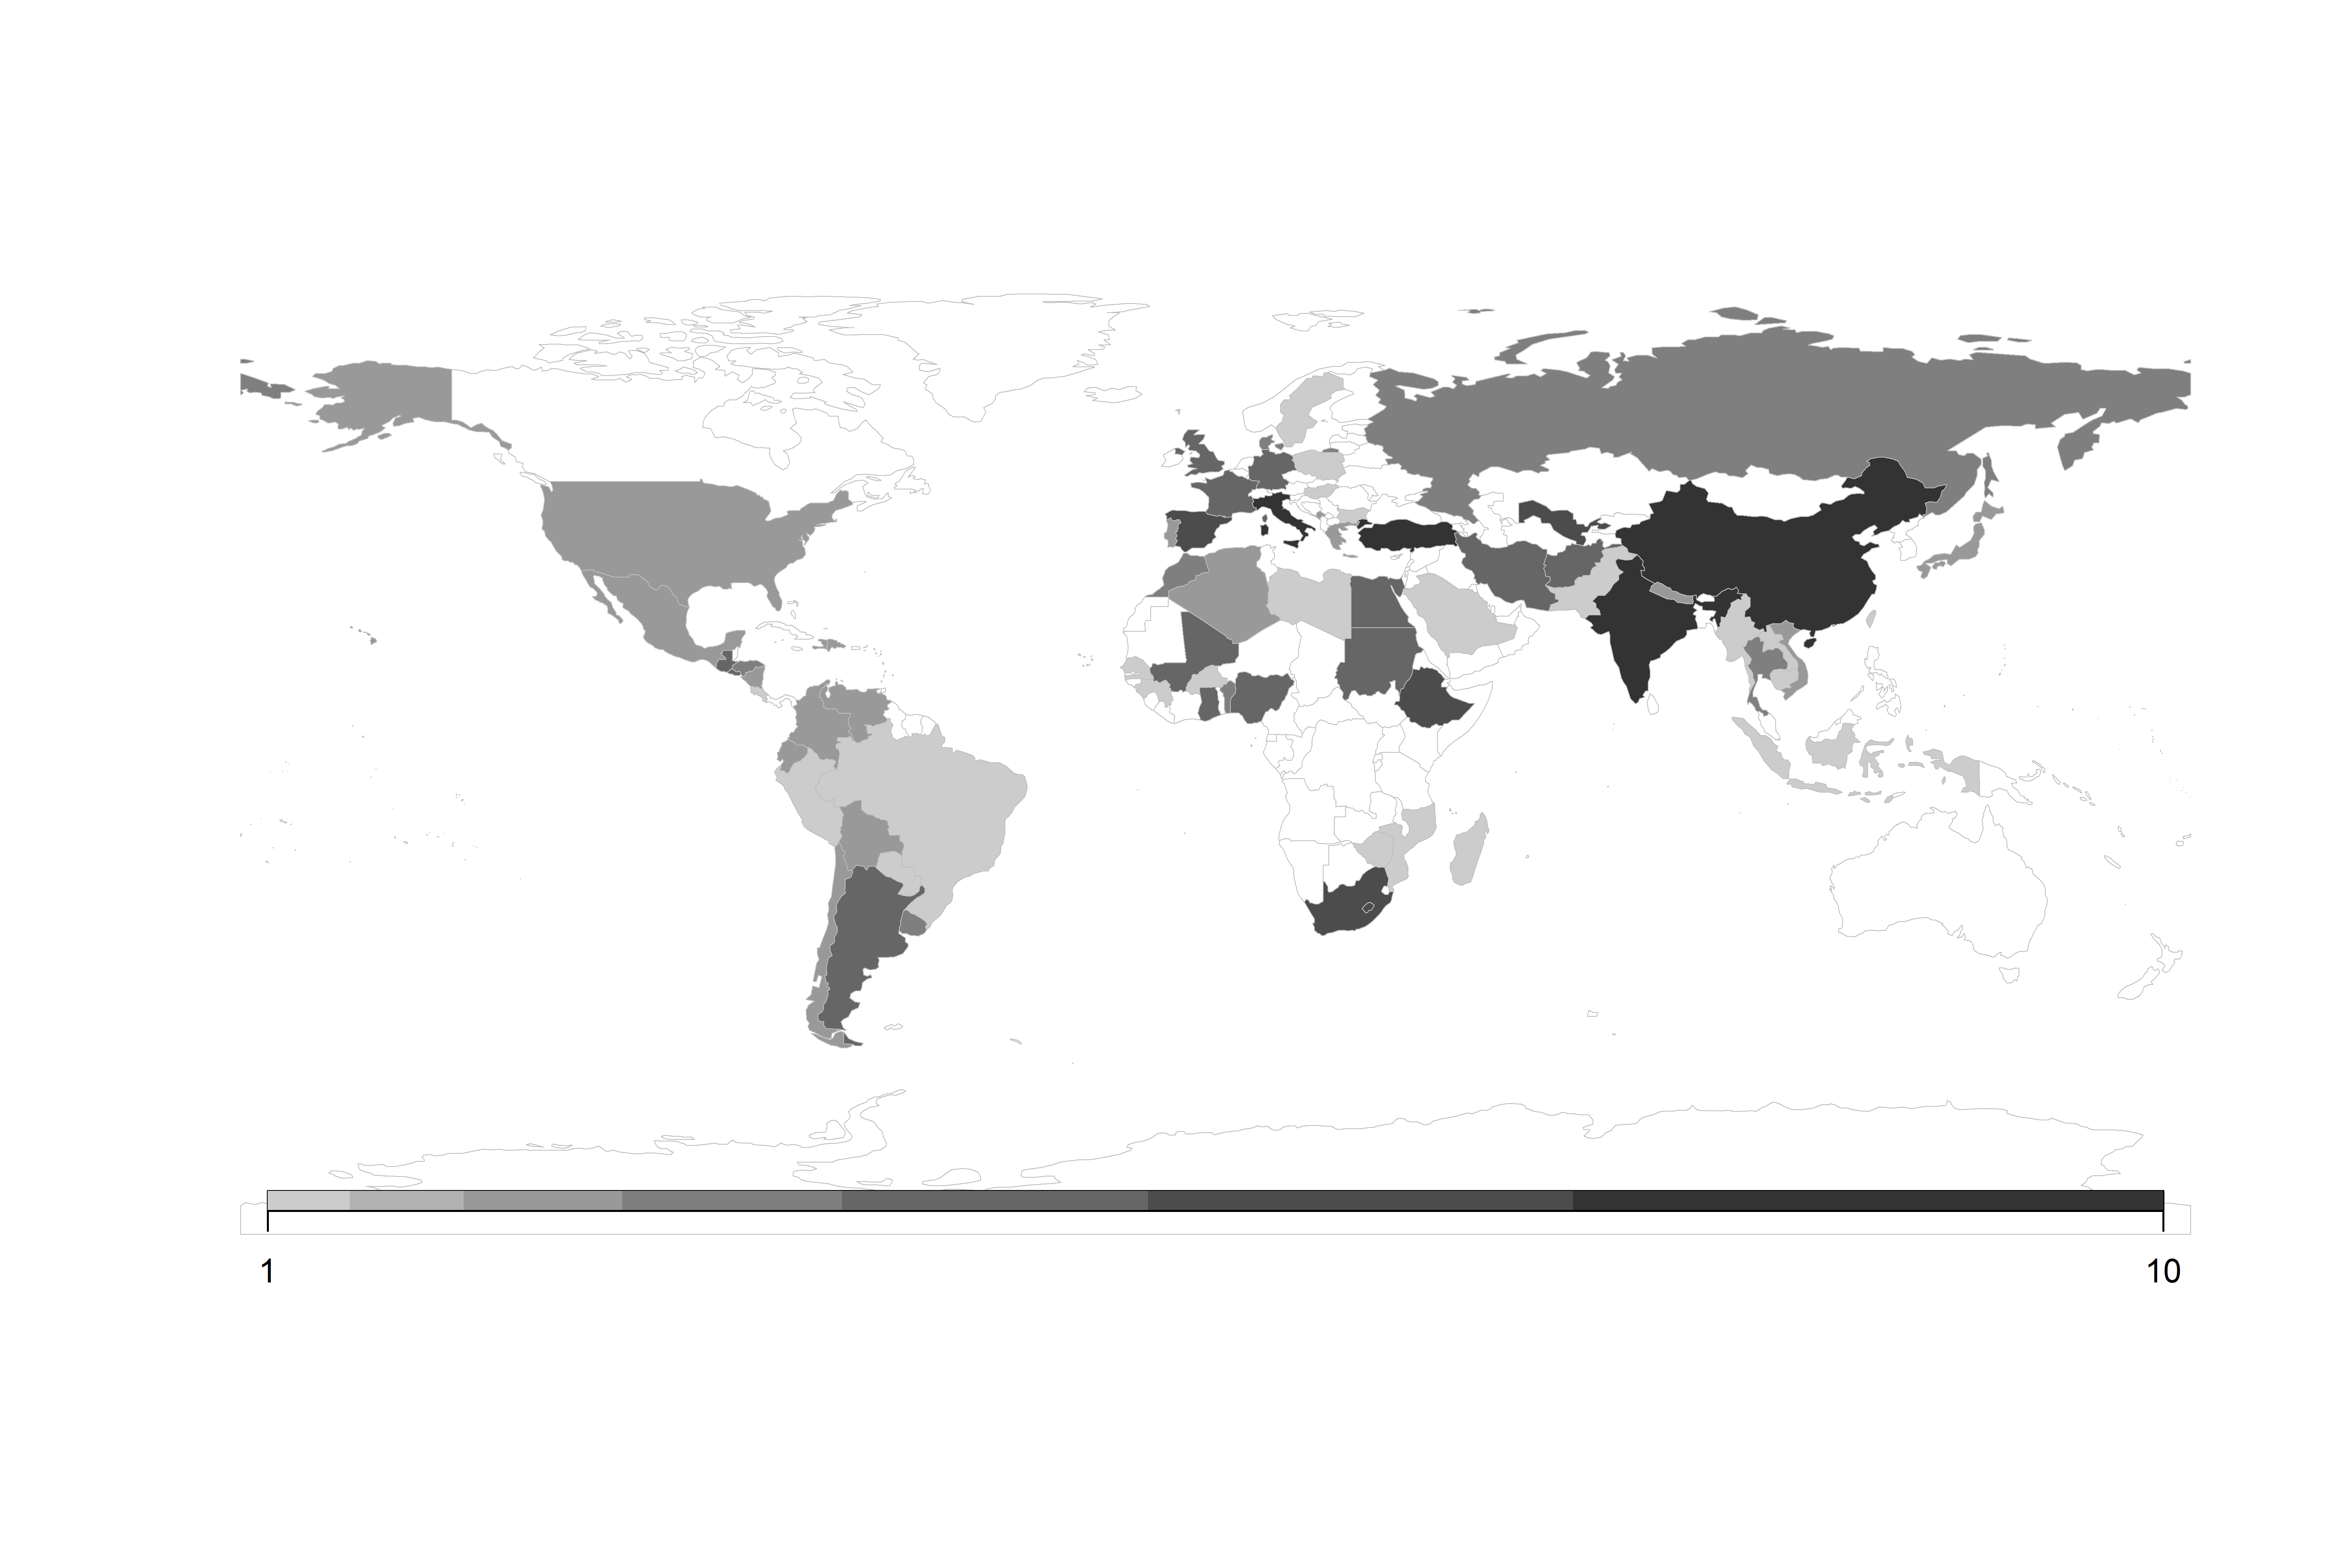
\includegraphics[width=\textwidth,
    height=\textheight, keepaspectratio]{img/historical_conflict_pm_map.png} \caption{Historical Conflict in Project Mars (logged), 1800-1900} \label{Fig: Mars_Map} \end{figure}


Table \ref{Tab: Hist_Conflict_Rob_Pm} shows the main results replacing the historical conflict indicator used in the main analysis with the indicator of 19th century wars from \citet{Lyall2020}. 

     \import{img/}{historical_conflict_robustness_pm}

\clearpage

\subsubsection{Conclusions}

The preceding discussion leads us to conclude that historical conflict does not confound our main results, at least as far as we can empirically test that with the measures available. More historical states \textit{are} correlated with more historical conflicts, but historical conflicts do not appear to be strongly correlated with modern armed conflicts. This is likely because wars in the past have conditional effects on state-building and future peace. Some wars, especially those in Europe, probably helped create cohesive, modern states that had overcome important state-building challenges prior to the 20th century. Here, past wars may be associated with future peace. But in other regions, primarily Africa, historical wars may have eroded trust between social groups that transmits into the modern world as weaker states and higher conflict risks \citep{Besley2014, Dincecco2019}. Our results reflect this - only in Africa do we find that historical conflict is correlated with modern conflict. Historical states may be correlated with historical wars, but they don't appear to be strongly correlated with modern wars. Nonetheless, when we do allow the impacts of war to vary by region, our main results hold up, suggesting that even in Africa, historical warfare and historical statehood may have different impacts on the propensity to modern conflict. 

\subsection{Table of cases}
 
 \import{img/}{anecdotesWithActors}
 
\clearpage 
\bibliographystyle{aspr}
\bibliography{../ArtificialBorders.bib}
\clearpage

